\subsection{Operations on complexes}

On the set A × A, the two operations

\[
\begin{array}{l} (a, b) + (a ^ {\prime}, b ^ {\prime}) = (a + a ^ {\prime}, b + b ^ {\prime}) \\ (a, b) (a ^ {\prime}, b ^ {\prime}) = (a a ^ {\prime}, a b ^ {\prime} + b a ^ {\prime}) \end{array}
\]

define a ring structure, denoted A(ε), with identity element 1 = (1, 0); the injection a ↦ (a, 0) = a1 allows A to be identified with a subring of A(ε); the module A(ε) is free with basis \{ 1, ε \} where ε = (0, 1); we have ε² = 0 and ε is central in A(ε).

When A is commutative, \(\mathrm{A}(\varepsilon)\) is a dual number algebra over A (III, p.~15). Endow \(\mathrm{A}(\varepsilon)\) with the ring grading (II, p.~164) for which \(\mathrm{A}(\varepsilon)_{0} = \mathrm{A}.1\) , \(\mathrm{A}(\varepsilon)_{-1} = \mathrm{A}. \varepsilon\) and \(\mathrm{A}(\varepsilon)_{n} = 0\) for \(n \neq 0, -1\) . It is clear that giving a structure of A-complex on a set C amounts to giving on C a structure of \(\mathrm{A}(\varepsilon)\) graded module, the differential d corresponding to the homothety \(\varepsilon_{C}\) ; likewise, morphisms of complexes correspond to graded homomorphisms of degree 0 of \(\mathrm{A}(\varepsilon)\) graded modules. The species of structure of \(\mathrm{A}(\varepsilon)\) graded modules and of A-complexes are therefore equivalent (E, IV, p.~9-10). We shall use this fact to transport to the theory of complexes the usual notions of the theory of graded modules.

To the notion of graded sub-A(ε)-module corresponds that of subcomplex: a subcomplex of the complex (C, d) is therefore a graded submodule C' of C such that, for every \(n \in Z\) , \(d_{n}(C_{n}') \subset C_{n-1}'\) ; if we denote by \(d'\) the graded A-homomorphism from C' to C' induced by d, then (C', d') is a complex structure, called the structure induced by (C, d). Unless expressly stated otherwise, every subcomplex will be equipped with the induced structure.

We leave it to the reader to similarly spell out the notions of quotient complex, exact sequence of complexes, kernel, cokernel, and image of a morphism of complexes, following the dictionary below:

graded quotient A(ε)-module

= quotient complex,

kernel, cokernel, image of a graded A(ε)-homomorphism of degree 0 \} kernel, cokernel, image of a morphism of complexes,

exact sequence of graded A(ε)-modules and graded homomorphisms of degree 0 \} = exact sequence of complexes.

For example, the canonical exact sequences of No. 1 give exact sequences of complexes, called canonical.

\begin{enumerate}
\def\labelenumi{(\Roman{enumi})}
\tightlist
\item
\end{enumerate}

\[
0 \longrightarrow \mathrm{Z} (\mathrm{C}) \longrightarrow \mathrm{C} \stackrel {\delta} {\longrightarrow} \mathrm{B} (\mathrm{C}) (- 1) \longrightarrow 0,\tag{II}
\]

\[
0 \longrightarrow \mathrm{B} (\mathrm{C}) \longrightarrow \mathrm{Z} (\mathrm{C}) \longrightarrow \mathrm{H} (\mathrm{C}) \longrightarrow 0,\tag{III}
\]

\[
0 \longrightarrow \mathrm{B} (\mathrm{C}) \longrightarrow \mathrm{C} \longrightarrow \mathrm{C} / \mathrm{B} (\mathrm{C}) \longrightarrow 0,\tag{IV}
\]

\[
0 \longrightarrow \mathrm{H} (\dot {\mathrm{C}}) \longrightarrow \mathrm{C} / \mathrm{B} (\mathrm{C}) \stackrel {\delta} {\longrightarrow} \mathrm{B} (\mathrm{C}) (- 1) \stackrel {\cdot} {\longrightarrow} 0,\tag{V}
\]

\[
0 \longrightarrow \mathrm{H} (\mathrm{C}) \longrightarrow \mathrm{C} / \mathrm{B} (\mathrm{C}) \longrightarrow \mathrm{Z} (\mathrm{C}) (- 1) \longrightarrow \mathrm{H} (\mathrm{C}) (- 1) \longrightarrow 0.
\]

Similarly, one defines the notions of direct sum of complexes, inductive system of complexes, and inductive limit of an inductive system of complexes.

Let \((\mathbf{C}_{i}, d_{i})\) be a family of complexes. One calls product of this family, and one denotes by \(\prod_{i \in I} (\mathbf{C}_{i}, d_{i})\), the complex \((\mathbf{C}, d)\) obtained as follows:

\begin{enumerate}
\def\labelenumi{\alph{enumi})}
\item
  for each \(n \in Z\) , \(C_{n}\) is the product A-module \(\prod_{i \in I} (\mathbf{C}_{i})_{n}\) of the homogeneous components \((\mathbf{C}_{i})_{n}\) of the given complexes,
\item
  for each \(n \in Z\) , \(d_{n} : C_{n} \to C_{n-1}\) is the A-homomorphism with components \((d_{i})_{n}\) .
\end{enumerate}

When I is finite, \(\prod_{i\in I}(\mathbf{C}_{i},d_{i})\) is equal to \(\bigoplus_{i\in I}(\mathbf{C}_{i},d_{i})\) One should note that, in general, the underlying A-module of the product complex \(\prod_{i\in I}(\mathbf{C}_{i},d_{i})\) is not the product A-module \(\prod_{i\in I}\mathbf{C}_{i}\) .

Consider a family (resp. a filtered inductive system) \((\mathbf{C}_i)_{i\in I}\) Let C be the direct sum (resp. the inductive limit) of \(C_i\) and let \(\alpha_{i}:C_{i}\to C\) the canonical homomorphisms. Then the \(\mathrm{H}(\alpha_{i}): \mathrm{H}(\mathrm{C}_{i})\to \mathrm{H}(\mathrm{C})\) define a graded homomorphism of degree 0, called canonical, from \(\bigoplus_{i\in I}\mathrm{H}(\mathrm{C}_{i})\) (resp. \(\varinjlim_{i\in I}\mathrm{H}(\mathrm{C}_{i})\) ) in \(\mathrm{H}(\mathrm{C})\) . Likewise, the canonical projections \(\prod_{i\in I}\mathrm{C}_{i}\to \mathrm{C}_{i}\) define a graded homomorphism of degree 0, called canonical, from \(\mathrm{H}(\prod \mathrm{C}_i)\) to \(\prod (\mathrm{H}(\mathrm{C}_i))\) .

PROPOSITION 1. --- For every family of complexes \((\mathbf{C}_{i})_{i\in I}\) , the canonical homomorphisms

\[
\bigoplus_ {i \in \mathbf {I}} \mathrm{H} (\mathrm{C} _ {i}) \rightarrow \mathrm{H} \left(\bigoplus_ {i \in \mathbf {I}} \mathrm{C} _ {i}\right), \quad \mathrm{H} \left(\prod_ {i \in \mathbf {I}} \mathrm{C} _ {i}\right)\rightarrow \prod_ {i \in \mathbf {I}} \mathrm{H} (\mathrm{C} _ {i})\tag{2}
\]

are bijective.

For every filtered inductive system of complexes \((\mathbf{C}_{i})_{i\in\mathbf{I}}\) , the canonical homomorphism

\[
\varinjlim_ {i \in \mathrm{I}} \mathrm{H} (\mathrm{C} _ {i}) \to \mathrm{H} (\varinjlim_ {i \in \mathrm{I}} \mathrm{C} _ {i})\tag{3}
\]

is bijective.

This follows immediately from II, p.~14, cor. 1 to prop. 7, p.~11, cor. to prop. 5, and p.~91, prop. 3.

\subsection{The connecting homomorphism and the exact homology sequence}

In this section, we consider an exact sequence of complexes

\[
0 \longrightarrow \mathrm{C} ^ {\prime} \stackrel {u} {\longrightarrow} \mathrm{C} \stackrel {v} {\longrightarrow} \mathrm{C} ^ {\prime \prime} \longrightarrow 0;
\]

denote by the same letter d the differentials of C, C' and C''\,'.

Let \(\Gamma\) be the set of \(x \in \mathbf{C}\) such that \(dx \in \operatorname{Im}(u)\) ; for \(x \in \Gamma\) , we have

\[
d \left(^ {- 1} u ^ {1} (d x)\right) = ^ {- 1} u ^ {1} (d d (x)) = 0,
\]

hence \(\overline{u}^{1}(dx)\in\mathbf{Z}(\mathbf{C}^{\prime})\) ; we also have \(dv(x)=v(dx)\in\operatorname{Im}(v\circ u)=0\) , hence \(v(x)\in\mathbf{Z}(\mathbf{C}^{\prime\prime})\) ; consider then the linear map \(\varphi:\Gamma\to\mathrm{H}(\mathbf{C}^{\prime\prime})\times\mathrm{H}(\mathbf{C}^{\prime})\) which maps every element \(x\in\Gamma\) to the class of \((v(x),\overline{u}^{1}(dx))\) .

Lemma 1. --- The image \(\varphi(\Gamma)\) of \(\Gamma\) in \(\mathrm{H}(\mathbf{C}^{\prime\prime}) \times \mathrm{H}(\mathbf{C}^{\prime})\) is the graph of a graded A-homomorphism of degree -1 of \(\mathrm{H}(\mathbf{C}^{\prime\prime})\) to \(\mathrm{H}(\mathbf{C}^{\prime})\) .

\begin{enumerate}
\def\labelenumi{\alph{enumi})}
\item
  If \(x \in \Gamma\) and if \(v(x) \in \mathbf{B}(\mathbf{C}'')\) , then \(\bar{u}^1(dx) \in \mathbf{B}(\mathbf{C}')\) : there exists indeed \(z'' \in \mathbf{C}''\) such that \(v(x) = dz''\) , then \(z \in \mathbf{C}\) such that \(z'' = v(z)\) , hence \(v(x) = v(dz)\) , then \(t' \in \mathbf{C}'\) such that \(x - dz = u(t')\) , which gives \(dx = u(dt')\) , hence \(\bar{u}^1(dx) = dt' \in \mathbf{B}(\mathbf{C}')\) .
\item
  Every element of \(\mathbf{Z}(\mathbf{C}^{\prime \prime})\) is the image under \(v\) of an element \(x\) of \(\mathbf{C}\) such that \(v(dx) = 0\) , i.e.~\(dx \in \operatorname{Im} u\) , that is, such that \(x \in \Gamma\) .
\item
  It follows from a) and b) that \(\varphi(\Gamma)\) is indeed a functional graph; since \(\varphi\) is bihomogeneous of bidegree \((0, -1)\) , this completes the proof.
\end{enumerate}

The graded homomorphism of degree -1 of H(C'') in H(C') thus defined is called the connecting homomorphism relative to the exact sequence (u, v); it is denoted \(\partial(u, v)\) or \(\partial_{u,v}\) or simply \(\partial\) . Its homogeneous components are denoted

\[
\partial_ {n} (u, v): \mathrm{H} _ {n} (\mathbf {C} ^ {\prime \prime}) \rightarrow \mathrm{H} _ {n - 1} (\mathbf {C} ^ {\prime}) \quad \text { and } \quad \partial^ {n} (u, v): \mathrm{H} ^ {n} (\mathbf {C} ^ {\prime \prime}) \rightarrow \mathrm{H} ^ {n + 1} (\mathbf {C} ^ {\prime}).
\]

By definition, to construct the image of a class \(\alpha\in\mathrm{H}_{n}(\mathbf{C}^{\prime\prime})\) by \(\partial\) we choose a cycle \(z^{\prime\prime}\in\mathbf{Z}_{n}(\mathbf{C}^{\prime\prime})\) in the class \(\alpha\) , then an element \(x\) of \(\mathbf{C}_{n}\) such that \(v(x)=z^{\prime\prime}\) ; then \(dx\) is of the form \(u(t')\) , \(t^{\prime}\in\mathbf{C}_{n-1}^{\prime}\) , and \(\partial(\alpha)\) is the homology class of \(t'\) .

In terms of correspondences, \(\partial_{n}(u,v)\) is therefore obtained from the correspondence \(u_{n-1}^{-1}\circ d_{n}\circ v_{n}^{-1}\) between \(\mathbf{C}_{n}^{\prime\prime}\) and \(\mathbf{C}_{n-1}^{\prime}\) , by passing to subsets \(\mathbf{Z}_{n}(\mathbf{C}^{\prime\prime})\) and \(\mathbf{Z}_{n-1}(\mathbf{C}^{\prime})\) , then to their quotients \(\mathbf{H}_{n}(\mathbf{C}^{\prime\prime})\) and \(\mathbf{H}_{n-1}(\mathbf{C}^{\prime})\) . This shows in particular that, if one replaces \(\mathbf{C},\mathbf{C}^{\prime},\mathbf{C}^{\prime\prime},u,v\) by \(\mathbf{C}(p),\mathbf{C}^{\prime}(p),\mathbf{C}^{\prime\prime}(p),u(p),v(p)\) , we have

\[
\partial (u (p), v (p)) = (- 1) ^ {p} \partial (u, v);\tag{4}
\]

likewise, if \(\lambda\) and \(\mu\) are two invertible elements of the center of A, one has

\[
\partial (\lambda u, \mu v) = \lambda^ {- 1} \mu^ {- 1} \partial (u, v).\tag{5}
\]

One can also relate \(\partial(u,v)\) to the snake diagram (X, p.~4). According to loc. cit., prop. 2, the sequences

\[
0 \longrightarrow Z _ {n} (C ^ {\prime}) \xrightarrow {Z _ {n} (u)} Z _ {n} (C) \xrightarrow {Z _ {n} (v)} Z _ {n} (C ^ {\prime \prime})
\]

and

\[
\mathrm{C} _ {n} ^ {\prime} / \mathrm{B} _ {n} (\mathrm{C} ^ {\prime}) \xrightarrow {\overline {{{u}}} _ {n}} \mathrm{C} _ {n} / \mathrm{B} _ {n} (\mathrm{C}) \xrightarrow {\overline {{{v}}} _ {n}} \mathrm{C} _ {n} ^ {\prime \prime} / \mathrm{B} _ {n} (\mathrm{C} ^ {\prime}) \longrightarrow 0,
\]

where \(\overline{u}_{n}\) and \(\overline{v}_{n}\) are deduced from \(u\) and \(v\) , are exact. Using the canonical exact sequences \((\mathrm{V}_{n})\) , one obtains a commutative diagram with exact rows and columns

\[
\begin{array}{c c c c} 0 & 0 & 0 \\ \downarrow & \mathrm{H} _ {n} (\mathrm{C} ^ {\prime}) & \xrightarrow {\mathrm{H} _ {n} (u)} & \mathrm{H} _ {n} (\mathrm{C}) \\ \downarrow & \mathrm{C} _ {n} ^ {\prime} / \mathrm{B} _ {n} (\mathrm{C} ^ {\prime}) & \xrightarrow {\bar {u} _ {n}} & \mathrm{C} _ {n} / \mathrm{B} _ {n} (\mathrm{C}) \\ \downarrow & 0 \longrightarrow Z _ {n - 1} (\mathrm{C} ^ {\prime}) & \xrightarrow {Z _ {n - 1} (u)} & Z _ {n - 1} (\mathrm{C}) \\ \downarrow & H _ {n - 1} (\mathrm{C} ^ {\prime}) & \xrightarrow {\mathrm{H} _ {n - 1} (u)} & H _ {n - 1} (\mathrm{C}) \\ \downarrow & 0 & 0 & 0 \end{array}
\]

The homomorphism \(\mathrm{H}_{n}(\mathbf{C}^{\prime \prime})\to \mathrm{H}_{n - 1}(\mathbf{C}^{\prime})\) associated with this diagram (loc. cit., prop. 2, (iii)) coincides by construction with \(\partial_n(u,v)\) . This also implies that the sequence of homomorphisms \((\mathrm{H}_n(u),\mathrm{H}_n(v),\partial_n(u,v),\mathrm{H}_{n - 1}(u),\mathrm{H}_{n - 1}(v))\) is exact; consequently:

THEOREM 1. --- The infinite sequence of homomorphisms of A-modules

\[
\begin{array}{r l} \dots & \to \mathrm{H} _ {n + 1} (\mathrm{C} ^ {\prime \prime}) \xrightarrow {\partial_ {n + 1} (u , v)} \mathrm{H} _ {n} (\mathrm{C} ^ {\prime}) \xrightarrow {\mathrm{H} _ {n} (u)} \mathrm{H} _ {n} (\mathrm{C}) \xrightarrow {\mathrm{H} _ {n} (v)} \mathrm{H} _ {n} (\mathrm{C} ^ {\prime \prime}) \\ & \xrightarrow {\partial_ {n} (u , v)} \mathrm{H} _ {n - 1} (\mathrm{C} ^ {\prime}) \xrightarrow {\mathrm{H} _ {n - 1} (u)} \mathrm{H} _ {n - 1} (\mathrm{C}) \xrightarrow {\mathrm{H} _ {n - 1} (v)} \mathrm{H} _ {n - 1} (\mathrm{C} ^ {\prime \prime}) \xrightarrow {\partial_ {n - 1} (u , v)} \mathrm{H} _ {n - 2} (\mathrm{C} ^ {\prime}) \to \dots \end{array}
\]

is exact.

This sequence is called the exact homology sequence associated with the exact sequence \((u, v)\) ; it is sometimes written in the form of an exact triangle of A-modules

\[
\begin{array}{c} \mathrm{H(C)} \\ \mathrm{H(u)} \nearrow \searrow \mathrm{H(v)} \\ \mathrm {H(C^ {\prime})} \xleftarrow [ \partial (u , v) ]{} \mathrm {H(C^{\prime\prime})}. \end{array}
\]

COROLLARY 1. --- If two of the complexes C, C', C'' have zero homology, then the third also has zero homology. For u (resp. v) to be a homologism, it is necessary and sufficient that C'' (resp. C') have zero homology. For \(\partial(u, v)\) to be bijective, it is necessary and sufficient that C have zero homology.

COROLLARY 2. --- Let u be a morphism of complexes. If Ker u and Coker u have zero homology, then u is a homologism.

Indeed, let \(u: \mathrm{E} \to \mathrm{E}'\) a morphism of complexes. If Ker \(u\) (resp. Coker \(u\) ) has zero homology, then the canonical morphism \(\mathrm{E} \to \operatorname{Im} u\) (resp. \(\operatorname{Im} u \to \mathrm{E}'\) ) is a homologism by Corollary 1.

PROPOSITION 2. — Consider a commutative diagram of complexes with exact rows

\[
\begin{array}{c} 0 \longrightarrow \mathrm{C} ^ {\prime} \stackrel {{u}} {{\longrightarrow}} \mathrm{C} \stackrel {{v}} {{\longrightarrow}} \mathrm{C} ^ {\prime \prime} \longrightarrow 0 \\ f ^ {\prime} \Big \downarrow \qquad \qquad \qquad f \Big \downarrow \qquad \qquad f ^ {\prime \prime} \Big \downarrow \\ 0 \longrightarrow \mathrm{C} _ {1} ^ {\prime} \stackrel {{u _ {1}}} {{\longrightarrow}} \mathrm{C} _ {1} \stackrel {{v _ {1}}} {{\longrightarrow}} \mathrm{C} _ {1} ^ {\prime \prime} \longrightarrow 0. \end{array}
\]

Then \(\mathbf{H}(f')\circ \partial (u,v) = \partial (u_1,v_1)\circ \mathbf{H}(f'')\)

Let \(\alpha'' \in \mathrm{H}(\mathbf{C}'')\) ; let \(z''\) be a cycle of class \(\alpha''\) and \(x\) an element of C such that \(v(x) = z''\) ; we have

\[
\begin{array}{r l} \big (\partial_ {u _ {1}, v _ {1}} \circ \mathrm{H} (f ^ {\prime \prime}) \big) (\alpha^ {\prime \prime}) = & \partial_ {u _ {1}, v _ {1}} (\overline {{f ^ {\prime \prime} (z ^ {\prime \prime})}}) = \overline {{u _ {1} ^ {- 1} (d f (x))}} = \overline {{f ^ {\prime} (u ^ {- 1} (d x))}} = \\ & = \mathrm{H} (f ^ {\prime}) (\overline {{u ^ {- 1} (d x)}}) = (\mathrm{H} (f ^ {\prime}) \circ \partial_ {u, v}) (\alpha^ {\prime \prime}). \end{array}
\]

Example. — Let C be a complex. Consider the canonical exact sequence

\[
0 \longrightarrow \mathrm{Z} (\mathrm{C}) \stackrel {j} {\longrightarrow} \mathrm{C} \stackrel {\delta} {\longrightarrow} \mathrm{B} (\mathrm{C}) (- 1) \longrightarrow 0,\tag{I}
\]

and let \(i: \mathbf{B}(\mathbf{C}) \to \mathbf{Z}(\mathbf{C})\) be the canonical injection. Then the connecting homomorphism \(\partial(j, \delta): \mathrm{H}(\mathrm{B}(\mathrm{C})) (-1) \to \mathrm{H}(\mathrm{Z}(\mathrm{C})) (-1)\) is identified with \(\mathrm{H}(i) (-1)\) , as one verifies immediately. Since \(\mathrm{H}(\delta) = 0\) , the exact homology sequence associated with (I) decomposes into the short exact sequences

\[
0 \longrightarrow \mathrm{B} _ {n} (\mathrm{C}) \stackrel {i} {\longrightarrow} Z _ {n} (\mathrm{C}) \stackrel {\mathrm{H} (j)} {\longrightarrow} \mathrm{H} _ {n} (\mathrm{C}) \longrightarrow 0.\tag{\((\mathrm{II}_{\mathfrak{n}})\)}
\]

* Applications:

\begin{enumerate}
\def\labelenumi{\arabic{enumi})}
\tightlist
\item
  Singular homology
\end{enumerate}

Let A be a ring. For every topological space X, one defines the singular complex C(X, A) of X with coefficients in A as follows:

In \(\mathbf{R}^{(N)}\) , let \((e_n)\) be the canonical basis; one calls canonical \(n\) -simplex the convex hull \(\Delta_n\) of \(\{e_0, \ldots, e_n\}\) . For \(i \in \{0, \ldots, n\}\) , one defines the affine map \(\iota_i: \Delta_{n-1} \to \Delta_n\) by \(\iota_i(e_k) = e_k\) for \(k < i\) and \(\iota_i(e_k) = e_{k+1}\) for \(k \geqslant i\) . One denotes by \(\mathbf{C}_n(\mathbf{X}, \mathbf{A})\) the A-module \(\mathbf{A}^{(\Sigma_n(\mathbf{X}))}\) , where \(\Sigma_n(\mathbf{X})\) is the set of continuous maps from \(\Delta_n\) to \(\mathbf{X}\) ; for \(n < 0\) , we set \(\mathbf{C}_n = 0\) . For \(i \in \{0, \ldots, n\}\) , one defines the linear map \(\partial_{n,i}: \mathbf{C}_n(\mathbf{X}, \mathbf{A}) \to \mathbf{C}_{n-1}(\mathbf{X}, \mathbf{A})\) by \(\partial_{n,i}(e_s) = e_{s \circ \iota_i}\) for \(s \in \Sigma_n(\mathbf{X})\) , and one sets \(d_n = \Sigma (-1)^t \partial_{n,i}\) . One verifies that

\[
\dots \mathrm{C} _ {n} (\mathrm{X}, \mathrm{A}) \xrightarrow {d _ {n}} \mathrm{C} _ {n - 1} (\mathrm{X}, \mathrm{A}) \rightarrow \dots
\]

is a complex. Its homology is called the singular homology of X with coefficients in A and is denoted H(X, A) or simply H(X).

If Y is a subspace of X, one denotes by C(X, Y, A) the quotient complex C(X, A)/C(Y, A), and by H(X, Y, A) its homology. It follows from Theorem I that one has an exact sequence:

\[
\dots \rightarrow \mathrm{H} _ {n} (\mathrm{Y}, \mathrm{A}) \rightarrow \mathrm{H} _ {n} (\mathrm{X}, \mathrm{A}) \rightarrow \mathrm{H} _ {n} (\mathrm{X}, \mathrm{Y}, \mathrm{A}) \rightarrow \mathrm{H} _ {n - 1} (\mathrm{Y}, \mathrm{A}) \rightarrow \mathrm{H} _ {n - 1} (\mathrm{X}, \mathrm{A}) \rightarrow \dots
\]

\begin{enumerate}
\def\labelenumi{\arabic{enumi})}
\setcounter{enumi}{1}
\tightlist
\item
  Finite cellular complexes
\end{enumerate}

Let X be a Hausdorff topological space. A finite cellular decomposition of X is given by an increasing sequence \((X_{n})_{n\in\mathbb{Z}}\) of closed subspaces of X satisfying the following conditions: (i) \(X_{n} = \varnothing\) for n \textless{} 0 ;

\begin{enumerate}
\def\labelenumi{(\roman{enumi})}
\setcounter{enumi}{1}
\item
  there exists an N such that \(X_{N} = X\) (hence \(X_{n} = X\) for n \textgreater{} N);
\item
  for all \(n\) , the space \(\mathbf{X}_{n} - \mathbf{X}_{n-1}\) has only finitely many connected components, called cells of dimension \(n\) ;
\item
  for every n, and for every connected component C of \(X_{n} - X_{n-1}\) there exists a homeomorphism of the open Euclidean ball \(\dot{B}_{n}\) of dimension n (TG, VI, p.~10) onto C which extends to a continuous map from the closed ball into X.
\end{enumerate}

One can show that these conditions imply that \(\mathbf{H}_n(\mathbf{X}_n, \mathbf{X}_{n-1}, \mathbf{A})\) is a free A-module \(\Gamma_n\) of rank equal to the number of cells of dimension \(n\) , and that \(\mathbf{H}_i(\mathbf{X}_n, \mathbf{X}_{n-1}, \mathbf{A}) = 0\) for \(i \neq n\) . We have \(\mathbf{C}(\mathbf{X}_n, \mathbf{X}_{n-1}, \mathbf{A}) = \mathbf{C}(\mathbf{X}_n, \mathbf{X}_{n-2}, \mathbf{A}) / \mathbf{C}(\mathbf{X}_{n-1}, \mathbf{X}_{n-2}, \mathbf{A})\) whence an exact sequence

\[
\mathrm{H} _ {n} \left(\mathrm{X} _ {n}, \mathrm{X} _ {n - 2}\right) \longrightarrow \mathrm{H} _ {n} \left(\mathrm{X} _ {n}, \mathrm{X} _ {n - 1}\right) \xrightarrow {d _ {n}} \mathrm{H} _ {n - 1} \left(\mathrm{X} _ {n - 1}, \mathrm{X} _ {n - 2}\right) \longrightarrow \mathrm{H} _ {n - 1} \left(\mathrm{X} _ {n}, \mathrm{X} _ {n - 2}\right),
\]

with a connecting homomorphism \(d_{n}:\Gamma_{n}\to\Gamma_{n-1}\) . We have \(d_{n}\circ d_{n+1}=0\) , which allows one to define a complex \(\Gamma:\cdots\to\Gamma_{n}\xrightarrow{d_{n}}\Gamma_{n-1}\to\cdots\) .

The exact sequence

\[
\mathrm{H} _ {n + 1} \left(\mathrm{X} _ {p}, \mathrm{X} _ {p - 1}\right)\rightarrow \mathrm{H} _ {n} \left(\mathrm{X} _ {p - 1}\right)\rightarrow \mathrm{H} _ {n} \left(\mathrm{X} _ {p}\right)\rightarrow \mathrm{H} _ {n} \left(\mathrm{X} _ {p}, \mathrm{X} _ {p - 1}\right)\rightarrow \mathrm{H} _ {n - 1} \left(\mathrm{X} _ {p - 1}\right)
\]

shows by induction on \(p\) that \(\mathrm{H}_{n}(\mathrm{X}_{p})=0\) for \(p<n\) , that \(\mathrm{H}_{n}(\mathrm{X}_{n})=\mathrm{Ker}\left(d_{n}:\Gamma_{n}\to\Gamma_{n-1}\right)\) and that \(\mathrm{H}_{n}(\mathrm{X}_{p})=\mathrm{H}_{n}(\Gamma)\) for \(p>n\) In particular \(\mathrm{H}_{n}(\mathrm{X})\) is identified with \(\mathrm{H}_{n}(\Gamma)\) .

Example. --- Consider the product of spheres \(\mathbf{S}_{2} \times \mathbf{S}_{2}\) and the complex projective space \(\mathbf{P}_{2}(\mathbf{C})\) . Let \(b \in \mathbf{S}_{2}\) ; one defines a cell decomposition \((\mathrm{Y}_{n})\) of \(\mathrm{Y} = \mathbf{S}_{2} \times \mathbf{S}_{2}\) by setting

\[
\mathrm{Y} _ {0} = \mathrm{Y} _ {1} = \{(b, b) \}, \quad \mathrm{Y} _ {2} = \mathrm{Y} _ {3} = (\{b \} \times \mathbf {S} _ {2}) \cup (\mathbf {S} _ {2} \times \{b \}) \quad \text {and} \quad \mathrm{Y} _ {4} = \mathbf {S} _ {2} \times \mathbf {S} _ {2};
\]

this decomposition has one cell of dimension 0, two of dimension 2, and one of dimension 4. The differentials of the associated complex are necessarily zero, hence \(\mathrm{H}_{0}(\mathrm{Y})\) , \(\mathrm{H}_{2}(\mathrm{Y})\) and \(\mathrm{H}_{4}(\mathrm{Y})\) are free of ranks 1, 2, and 1 respectively, and \(\mathrm{H}_{n}(\mathrm{Y}) = 0\) for \(n \notin \{0, 2, 4\}\) .

We obtain a cellular decomposition \((\mathbf{Z}_{n})\) of \(\mathbf{P}_{2}(\mathbf{C})\) by setting

\[
\mathbf {Z} _ {0} = \mathbf {Z} _ {1} = \{c \}, \quad \mathbf {Z} _ {2} = \mathbf {Z} _ {3} = \mathbf {P} _ {1} (\mathbf {C}), \quad \mathbf {Z} _ {4} = \mathbf {P} _ {2} (\mathbf {C}),
\]

the space \(\mathbf{P}_{1}(\mathbf{C})\) being embedded in \(\mathbf{P}_{2}(\mathbf{C})\) (TG, VIII, p.~20), and \(c\) being a point of \(\mathbf{P}_{1}(\mathbf{C})\) ; this decomposition has one cell of dimension 0, one of dimension 2, and one of dimension 4. Here again the differentials of the complex are necessarily zero, and it follows that \(\mathbf{H}_{n}(\mathbf{P}_{2}(\mathbf{C}))\) is isomorphic to A for \(n \in \{0, 2, 4\}\) and 0 otherwise.

Since the homology modules in degree 2 of the two spaces under consideration are free of rank 2 and 1, respectively, these spaces are not homeomorphic. *

\subsection{Homotopies}

DEFINITION 4. --- Let (C, d) and (C', d') be two complexes, and let f and g be two morphisms from C to C'. A homotopy connecting f to g is any graded A-homomorphism s of degree 1 from C to C' such that \(g - f = d' \circ s + s \circ d\) .

We say that f and g are homotopic if there exists a homotopy connecting f to g.

If \(h\) is a third morphism of \(C\) to \(C'\) and if \(s\) (resp. \(t\) ) is a homotopy connecting \(f\) to \(g\) (resp. \(g\) to \(h\) ), then \(s + t\) is a homotopy connecting \(f\) to \(h\) ; consequently, the relation “f and g are two homotopic morphisms from C to C'” is an equivalence relation, whose classes are called the homotopy classes of morphisms from C to C'.

Given two topological spaces X and Y, and a continuous map \(f: \mathbf{X} \to \mathbf{Y}\) , we define a linear map \(f_{*}\) of the singular complex (cf.~no. 3) C(X, A) into C(Y, A) by setting \(f_{*}(e_{s}) = e_{f \circ s}\) for \(s \in \Sigma_{n}(\mathbf{X})\) . This map is a morphism of complexes.

Two continuous maps \(f\) and \(g\) from X to Y are said to be topologically homotopic if there exists a continuous map \(h\) of \([0, 1] \times X\) into Y such that \(h(0, x) = f(x)\) and \(h(1, x) = g(x)\) for all \(x \in X\) . We show that, if \(f\) and \(g\) are topologically homotopic, the morphisms \(f_*\) and \(g_*\) are homotopic in the sense of Definition 4 above. It is this fact that is the origin of the terminology used in algebra. *

PROPOSITION 3. --- If f and g are two homotopic morphisms from C to C', then H(f) = H(g).

Let s be a homotopy connecting f to g. We have

\[
(g - f) (\mathbf {Z} (\mathbf {C})) = (d ^ {\prime} \circ s + s \circ d) (\mathbf {Z} (\mathbf {C})) = (d ^ {\prime} \circ s) (\mathbf {Z} (\mathbf {C})) \subset \mathrm{B} (\mathbf {C} ^ {\prime}),
\]

hence \(\mathrm{H}(g - f) = 0\) and \(\mathrm{H}(g) = \mathrm{H}(f)\) .

COROLLARY. --- A morphism homotopic to a homologism is a homologism.

PROPOSITION 4. --- Let C, C', D, D' be four complexes, \(f: \mathbf{C} \to \mathbf{C}'\) , \(g: \mathbf{C} \to \mathbf{C}'\) , \(u: \mathbf{D} \to \mathbf{C}\) , \(v: \mathbf{C}' \to \mathbf{D}'\) four morphisms. If s is a homotopy relating \(f\) to \(g\) , then \(v \circ s \circ u\) is a homotopy connecting \(v \circ f \circ u\) to \(v \circ g \circ u\) . If f and g are homotopic, then so are \(v \circ f \circ u\) and \(v \circ g \circ u\) .

That is clear.

COROLLARY. --- Let C, C′, C″ be three complexes, and f and g two morphisms from C to C′, \(f_{1}\) and \(g_{1}\) two morphisms from C' to C''. If s and \(s_{1}\) are homotopies connecting f to g and \(f_{1}\) to \(g_{1}\) respectively, then \(s_{1} \circ f + g_{1} \circ s\) is a homotopy connecting \(f_{1} \circ f\) to \(g_{1} \circ g\) . If f and \(f_{1}\) are homotopic to g and \(g_{1}\) respectively, then \(f_{1} \circ f\) is homotopic to \(g_{1} \circ g\) .

Indeed, \(s_{1} \circ f\) connects \(f_{1} \circ f\) to \(g_{1} \circ f\) and \(g_{1} \circ s\) connects \(g_{1} \circ f\) to \(g_{1} \circ g\) .

DEFINITION 5. --- A morphism of complexes \(f: \mathbb{C} \to \mathbb{C}'\) is called a homotopy equivalence if there exists a morphism \(f': \mathbb{C}' \to \mathbb{C}\) such that \(f' \circ f\) and \(f \circ f'\) are homotopic to \(1_{\mathbb{C}}\) and \(1_{\mathbb{C}'}\) respectively.

It is clear that \(f'\) is then also a homotopy equivalence; one also says that \(f'\) is the inverse of \(f\) up to homotopy. If \(f'\) and \(f_1'\) are both inverses of \(f\) up to homotopy, then \(f'\) and \(f_1'\) are homotopic (indeed, by the preceding corollary, \(f_1' = f_1' \circ 1_{\mathbf{C}'}\) is homotopic to \(f_1' \circ f \circ f'\) , hence to \(1_{\mathbf{C}} \circ f' = f'\) ).

PROPOSITION 5. — A homotopism is a homologism; a morphism composed of homotopisms is a homotopism. A morphism homotopic to a homotopism is a homotopism.

Let \(f: \mathbf{C} \to \mathbf{C}'\) and \(f_1: \mathbf{C}' \to \mathbf{C}''\) be homotopisms of complexes, \(f': \mathbf{C}' \to \mathbf{C}\) and \(f_1': \mathbf{C}'' \to \mathbf{C}'\) morphisms inverse up to homotopy. We have

\[
\mathrm{H} (f ^ {\prime}) \circ \mathrm{H} (f) = \mathrm{H} (f ^ {\prime} \circ f) = \mathrm{H} (1 _ {\mathrm{C}}) = 1 _ {\mathrm{H(C)}} \quad (\text { prop. } 3)
\]

and likewise \(\mathrm{H}(f) \circ \mathrm{H}(f') = 1_{\mathrm{H}(\mathbb{C}')}\) , hence \(\mathrm{H}(f)\) is bijective and \(f\) is a homologism. On the other hand, \((f' \circ f_1') \circ (f_1 \circ f)\) is homotopic to \(f' \circ 1_{\mathbb{C}'} \circ f\) (prop. 4), hence to \(1_{\mathbb{C}}\) ; similarly, \((f_1 \circ f) \circ (f' \circ f_1')\) is homotopic to \(1_{\mathbb{C}''}\) and \(f_1 \circ f\) is a homotopism. Finally, if \(g: \mathbb{C} \to \mathbb{C}'\) is a morphism homotopic to \(f\) , \(f' \circ g\) is homotopic to \(f' \circ f\) , hence to \(1_{\mathbb{C}}\) ; similarly, \(g \circ f'\) is homotopic to \(f \circ f'\) , hence to \(1_{\mathbb{C}'}\) and \(g\) is a homotopism.

COROLLARY. --- Let C, C', D, D' be four complexes, \(f: \mathbf{C} \to \mathbf{C}'\) a morphism, \(u: \mathbf{D} \to \mathbf{C}\) and \(v: \mathbf{C}' \to \mathbf{D}'\) homotopisms. In order that \(v \circ f \circ u\) be a homotopism (resp. a homologism), it is necessary and sufficient that \(f\) be one.

If \(f\) is a homotopism (resp. a homologism), then \(v \circ f \circ u\) is composed of homotopisms (resp. homologisms), hence is one. Conversely, let \(\overline{u}\) and \(\overline{v}\) be morphisms inverse to \(u\) and \(v\) up to homotopy; then \(\overline{v} \circ (v \circ f \circ u) \circ \overline{u}\) is homotopic to \(f\) by prop. 4; whence the conclusion by prop. 5, and the corollary of prop. 3.

We say that the complex C is homotopic to zero if \(1_{C}\) is homotopic to the zero map, that is, if there exists a graded A-endomorphism s of degree 1 of C such that \(1_{C} = s \circ d + d \circ s\) . This also amounts to saying that the unique morphism \(0 \to C\) (resp. \(C \to 0\) ) is a homotopism. A complex homotopic to zero has zero homology (prop. 5).

Example. --- Let \(u: \mathbf{M} \to \mathbf{N}\) and \(v: \mathbf{N} \to \mathbf{P}\) be homomorphisms of A-modules such that \(v \circ u = 0\) ; let C be the complex such that \(\mathbf{C}_2 = \mathbf{M}\) , \(\mathbf{C}_1 = \mathbf{N}\) , \(\mathbf{C}_0 = \mathbf{P}\) , \(\mathbf{C}_i = 0\) for \(i \neq 0, 1, 2, d_2 = u, d_1 = v, d_i = 0\) for \(i \neq 1, 2\) . Then C has zero homology if and only if the sequence \(0 \to \mathbf{M} \xrightarrow{u} \mathbf{N} \xrightarrow{v} \mathbf{P} \to 0\) is exact. It is homotopic to zero if and only if this sequence is split. Indeed, saying that C is homotopic to zero means that there exist A-homomorphisms \(s: \mathbf{P} \to \mathbf{N}\) and \(t: \mathbf{N} \to \mathbf{M}\) such that \(v \circ s = 1_{\mathbf{P}}, s \circ v + u \circ t = 1_{\mathbf{N}}, t \circ u = 1_{\mathbf{M}}\) ; this implies that the sequence is split; conversely, if \(s\) is an A-linear section of \(v\) , we define \(t\) by \(u \circ t = 1_{\mathbf{N}} - s \circ v\) , which is possible since \(v \circ (1_{\mathbf{N}} - s \circ v) = v - v \circ s \circ v = 0\) .

\subsection{Split complexes}

PROPOSITION 6. — Let (C, d) be a complex. The following conditions are equivalent:

\begin{enumerate}
\def\labelenumi{(\roman{enumi})}
\item
  there exists a homotopism from (C, d) to (H(C), 0)
\item
  there exists a graded A-endomorphism s of C, of degree 1, such that \(d = d \circ s \circ d\) ;
\item
  B(C) and Z(C) are direct summands of C;
\item
  (C, d) is a direct sum of subcomplexes that are either of length 0, or of length 1 with zero homology.
\item
  \(\Rightarrow\) (ii): let \(\varphi: \mathbf{C} \to \mathbf{H}(\mathbf{C})\) be a homotopism; there then exists a morphism of complexes \(\psi: \mathbf{H}(\mathbf{C}) \to \mathbf{C}\) and an endomorphism \(s\) of \(\mathbf{C}\) of degree 1 such that \(\psi \circ \varphi = 1_{\mathbf{C}} - s \circ d - d \circ s\) . We have \(d \circ \psi = \psi \circ 0 = 0\) , hence
\end{enumerate}

\[
0 = d \circ \psi \circ \varphi = d - d \circ s \circ d - d \circ d \circ s = d - d \circ s \circ d, \quad \text {whence (ii)}.
\]

\begin{enumerate}
\def\labelenumi{(\roman{enumi})}
\setcounter{enumi}{1}
\item
  \(\Rightarrow\) (iii): let \(s\) be as in (ii). Then \(d \circ (1_{\mathbb{C}} - s \circ d) = 0\) , hence \(1_{\mathbb{C}} - s \circ d\) is a projector of \(\mathbf{C}\) onto \(\mathbf{Z}(\mathbf{C})\) , and \((d \circ s) \circ d = d\) , hence \(d \circ s\) is a projector of \(\mathbf{C}\) onto \(\mathbf{B}(\mathbf{C})\) .
\item
  \(\Rightarrow\) (iv): for each \(n\in\mathbf{Z}\) , set \(Z_{n}=Z_{n}(\mathrm{C})\) , \(B_{n}=B_{n}(\mathrm{C})\) and choose submodules \(K_{n}\) and \(B_{n}^{\prime}\) of \(C_{n}\) such that \(C_{n}=B_{n}^{\prime}\oplus Z_{n}\) , \(Z_{n}=K_{n}\oplus B_{n}\) . Then
\end{enumerate}

\[
\mathrm{E} _ {(n)} = \mathrm{K} _ {n} (- n) \quad \text { and } \quad \mathrm{F} _ {(n)} = \mathrm{B} _ {n} ^ {\prime} (- n) \oplus \mathrm{B} _ {n - 1} (1 - n)
\]

are subcomplexes of (C, d); we have (C, d) = \(\bigoplus_{n \in \mathbf{Z}} (\mathrm{E}_{(n)} \oplus \mathrm{F}_{(n)})\) ; each \(\mathrm{E}_{(n)}\) is either zero or of length 0, each \(\mathrm{F}_{(n)}\) is either zero or of length 1 and with zero homology, whence (iv).

\begin{enumerate}
\def\labelenumi{(\roman{enumi})}
\setcounter{enumi}{3}
\tightlist
\item
  \(\Rightarrow\) (i): it suffices to note that (i) is satisfied when C is of length zero, or of zero homology and length 1.
\end{enumerate}

DEFINITION 6. --- A complex C is said to be split if it satisfies the equivalent conditions of prop. 6.

An endomorphism s of C satisfying condition (ii) of prop. 6 is called a splitting of C.

Examples. --- 1) A complex with zero differential is split.

\begin{enumerate}
\def\labelenumi{\arabic{enumi})}
\setcounter{enumi}{1}
\item
  The complexes homotopic to zero are the split complexes with zero homology, i.e.~the complexes C such that H(C) = 0 and Z(C) is a direct summand of C.
\item
  Let \(f: \mathbf{M} \to \mathbf{N}\) be a homomorphism of A-modules and C the complex such that \(\mathbf{C}_1 = \mathbf{M}, \mathbf{C}_0 = \mathbf{N}, \mathbf{C}_i = 0\) for \(i \neq 0, 1, d_1 = f, d_i = 0\) for \(i \neq 1\) . Then C is split if and only if Ker \(f\) is a direct summand of M and Im \(f\) a direct summand of N.
\item
  The complex C is split as soon as B(C) and H(C) are projective (resp. as soon as \(B_{n}(C)\) and \(H_{n}(C)\) are injective for each n). Indeed, by the exact sequences \((I_{n})\) to \((IV_{n})\) of no. 1, Z(C) is then a direct summand of C and B(C) a direct summand of Z(C) (resp. B(C) is a direct summand of C and Z(C)/B(C) a direct summand of C/B(C)).
\item
  In particular, if A is principal, a free complex C is split if and only if H(C) is free (that is, H \(_{n}\) (C) free for every n ∈ Z).
\end{enumerate}

Remark. --- a) Suppose that the canonical exact sequence of graded A-modules

\[
0 \to \mathrm{B} (\mathrm{C}) \to \mathrm{Z} (\mathrm{C}) \xrightarrow {\pi} \mathrm{H} (\mathrm{C}) \to 0\tag{II}
\]

is split (this holds for example if H(C) is projective, or B \(_{n}\) (C) injective for each n); let σ : H(C) → Z(C) be a graded A-linear section of π, and let ψ be the homomorphism x ↦ σ(x) from H(C) to C. Then ψ is a homologism from (H(C), 0) to C, such that H(ψ) = 1 \(_{H(C)}\) .

\begin{enumerate}
\def\labelenumi{\alph{enumi})}
\setcounter{enumi}{1}
\tightlist
\item
  Suppose that the canonical exact sequence of graded A-modules
\end{enumerate}

\[
0 \rightarrow \mathrm{H} (\mathrm{C}) \stackrel {i} {\rightarrow} \mathrm{C} / \mathrm{B} (\mathrm{C}) \rightarrow \mathrm{B} (\mathrm{C}) (- 1) \rightarrow 0\tag{IV}
\]

is split (this occurs, for example, if B(C) is projective, or H \(_{n}\) (C) is injective for each \(n\) ); let \(\tau: \mathbf{C} / \mathbf{B}(\mathbf{C}) \to \mathbf{H}(\mathbf{C})\) be a graded A-linear retraction of \(i\) and \(\varphi\) the homomorphism from C to \(\mathbf{H}(\mathbf{C})\) which associates to each element of C the image under \(\tau\) of its class modulo \(\mathbf{B}(\mathbf{C})\) . Then \(\varphi\) is a homologism from C to \((\mathbf{H}(\mathbf{C}), 0)\) such that \(\mathbf{H}(\varphi) = 1_{\mathbf{H}(\mathbf{C})}\) .

\subsection{Cone and cylinder of a morphism of complexes}

Let \(u:(\mathbf{C}^{\prime},d^{\prime})\to(\mathbf{C},d)\) be a morphism of complexes. Let \(\operatorname{Cyl}(u)\) and \(\operatorname{Con}(u)\) be the \(\text{graded A-modules }\operatorname{Cyl}(u)=\mathbf{C}^{\prime}\oplus\mathbf{C}^{\prime}(-1)\oplus\mathbf{C}\) , \(\operatorname{Con}(u)=\mathbf{C}^{\prime}(-1)\oplus\mathbf{C}\) and let us define graded A-linear maps of degree \((-1)\)

\(\overline{\mathbf{D}}:\operatorname {Cyl}(u)\to \operatorname {Cyl}(u),\quad \overline{\mathbf{D}} (x^{\prime},y^{\prime},x) = (d^{\prime}x^{\prime} + y^{\prime}, - d^{\prime}y^{\prime},dx - u(y^{\prime})),\)

D : Con \((u) \to \text{Con}(u)\) , D \((y', x) = (-d'y', dx - u(y'))\) .

(Here, and in what follows, we denote by \(x\) , \(y\) , \ldots{} arbitrary elements of C, \(x'\) , \(y'\) , \ldots{} arbitrary elements of C'.)

Lemma 2. --- (Cyl \((u)\) , \(\overline{\mathbf{D}}\) ) and (Con \((u)\) , D) are complexes of A-modules.

Indeed, we have

\[
\begin{array}{r l} \overline {{\mathbf {D}}} \circ \overline {{\mathbf {D}}} (x ^ {\prime}, y ^ {\prime}, x) & = \overline {{\mathbf {D}}} (d ^ {\prime} x ^ {\prime} + y ^ {\prime}, - d ^ {\prime} y ^ {\prime}, d x - u (y ^ {\prime})) = \\ & = (d ^ {\prime} (d ^ {\prime} x ^ {\prime} + y ^ {\prime}) - d ^ {\prime} y ^ {\prime}, - d ^ {\prime} (- d ^ {\prime} y ^ {\prime}), d (d x - u (y ^ {\prime})) - u (- d ^ {\prime} y ^ {\prime})) = 0 \end{array}
\]

since \(d' \circ d' = 0\) , \(d \circ d = 0\) and \(d \circ u = u \circ d'\) . Likewise \(D \circ D = 0\) .

DEFINITION 7. --- The complexes Cyl (u) and Con (u) are called respectively the cylinder and the cone of the morphism u.

Example. --- Let \(u: \mathbf{M} \to \mathbf{N}\) be a homomorphism of A-modules; then the only nonzero homogeneous components of \(\operatorname{Cyl}(u)\) and \(\operatorname{Con}(u)\) are

\[
\operatorname{Cyl} _ {1} (u) = \mathrm{M}, \quad \operatorname{Cyl} _ {0} (u) = \mathrm{M} \oplus \mathrm{N},
\]

\[
\operatorname{Con} _ {1} (u) = \mathrm{M}, \quad \operatorname{Con} _ {0} (u) = \mathrm{N},
\]

and we have \(\overline{\mathrm{D}}(m) = (m, -u(m))\) , \(\mathrm{D}(m) = -u(m)\) for \(m \in \mathbf{M}\) ; consequently,

\[
\mathrm{H} _ {1} (\text { Con } (u)) = \operatorname{Ker} (u), \quad \mathrm{H} _ {0} (\text { Con } (u)) = \operatorname{Coker} (u).
\]

The complex \(\Gamma(s)\) associated with the space \(\{s\}\) endowed with its unique cellular decomposition is reduced to the module A and is identified with a subcomplex of \(\Gamma(\text{Con}(f))\) ; denote by \(\Gamma(\text{Con}(f), s)\) the quotient complex. The map \(f\) defines a morphism of complexes \(\Gamma(f): \Gamma(X) \to \Gamma(Y)\) , and one can show that the complexes \(\Gamma(\text{Cyl}(f))\) and \(\Gamma(\text{Con}(f), s)\) are respectively identified with \(\text{Cyl}(\Gamma(f))\) and \(\text{Con}(\Gamma(f))\) .

Moreover, and without any hypotheses on X and Y, one associates to \(f\) a morphism of complexes \(f_{*}: \mathrm{C}(\mathrm{X}, \mathrm{A}) \to \mathrm{C}(\mathrm{Y}, \mathrm{A})\) . One can construct injective homotopisms from \(\mathrm{Cyl}(f_{*})\) to \(\mathrm{C}(\mathrm{Cyl}(f), \mathrm{A})\) and from \(\mathrm{Con}(f_{*})\) to \(\mathrm{C}(\mathrm{Con}(f), \{s\}, \mathrm{A})\) .

Let \(\tilde{f}: X \to \text{Cyl}(f)\) be the map which to \(x\) associates the image of \((0, x)\) , \(\alpha: Y \to \text{Cyl}(f)\) the canonical map and \(\beta: \text{Cyl}(f) \to Y\) the map which associates \(y\) to its image in \(\text{Cyl}(f)\) for \(y \in Y\) and \(f(x)\) to the image of \((t, x)\) in \(\text{Cyl}(f)\) for \(t \in [0, 1]\) and \(x \in X\) . The map \(\tilde{f}\) is a homeomorphism from \(X\) onto a closed subset of \(\text{Cyl}(f)\) , we have \(\beta \circ \alpha = \text{Id}_Y\) , and \(\alpha \circ \beta\) is topologically homotopic to the identity of \(\text{Cyl}(f)\) . These properties are to be compared with Proposition 7 below.

Consider now the graded A-linear maps of degree 0

\[
\tilde {u}: \mathrm{C} ^ {\prime} \rightarrow \operatorname{Cyl} (u), \quad \tilde {u} (x ^ {\prime}) = (x ^ {\prime}, 0, 0),
\]

\[
\alpha : \mathrm{C} \rightarrow \operatorname{Cyl} (u), \quad \alpha (x) = (0, 0, x),
\]

\[
\beta : \operatorname{Cyl} (u) \rightarrow \mathrm{C}, \quad \beta \left(x ^ {\prime}, y ^ {\prime}, x\right) = u \left(x ^ {\prime}\right) + x,
\]

\[
\pi : \mathbf {C} \rightarrow \operatorname{Con} (u), \quad \pi (x) = (0, x),
\]

\[
\tilde {\pi}: \operatorname{Cyl} (u) \to \operatorname{Con} (u), \quad \tilde {\pi} (x ^ {\prime}, y ^ {\prime}, x) = (y ^ {\prime}, x),
\]

\[
\delta : \operatorname{Con} (u) \to \mathbf {C} ^ {\prime} (- 1), \qquad \delta (y ^ {\prime}, x) = y ^ {\prime}.
\]

PROPOSITION 7. --- a) The maps \(\tilde{u}, \alpha, \beta, \pi, \tilde{\pi}, \delta\) are morphisms of complexes: we have \(u = \beta \circ \tilde{u}, \pi = \tilde{\pi} \circ \alpha, \beta \circ \alpha = 1_{\mathbb{C}}\) .

\begin{enumerate}
\def\labelenumi{\alph{enumi})}
\setcounter{enumi}{1}
\tightlist
\item
  The sequences of morphisms of complexes
\end{enumerate}

\begin{enumerate}
\def\labelenumi{(\arabic{enumi})}
\setcounter{enumi}{5}
\tightlist
\item
\end{enumerate}

\[
0 \rightarrow \mathrm{C} ^ {\prime} \stackrel {\tilde {u}} {\rightarrow} \operatorname{Cyl} (u) \stackrel {\tilde {\pi}} {\rightarrow} \operatorname{Con} (u) \rightarrow 0\tag{7}
\]

\[
0 \rightarrow \mathrm{C} \xrightarrow {\pi} \operatorname{Con} (u) \xrightarrow {\delta} \mathrm{C} ^ {\prime} (- 1) \rightarrow 0
\]

are exact.

\begin{enumerate}
\def\labelenumi{\alph{enumi})}
\setcounter{enumi}{2}
\tightlist
\item
  The morphisms \(\alpha : \mathbf{C} \to \operatorname{Cyl}(u)\) and \(\beta : \operatorname{Cyl}(u) \to \mathbf{C}\) are mutually inverse homotopisms up to homotopy.
\end{enumerate}

Assertion a) is equivalent to the formulas

\[
\tilde {u} \circ d ^ {\prime} = \overline {{\mathbf {D}}} \circ \tilde {u}, \alpha \circ d = \overline {{\mathbf {D}}} \circ \alpha , \beta \circ \overline {{\mathbf {D}}} = d \circ \beta , \pi \circ d = \mathbf {D} \circ \pi ,
\]

\[
\tilde {\pi} \circ \overline {{\mathbf {D}}} = \mathbf {D} \circ \tilde {\pi}, \delta \circ \mathbf {D} = - d ^ {\prime} \circ \delta , u = \beta \circ \tilde {u}, \pi = \tilde {\pi} \circ \alpha , \beta \circ \alpha = 1 _ {\mathrm{c}}
\]

which are verified by immediate calculations. Assertion b) is trivial. Let us prove c); on the one hand one has \(\beta \circ \alpha = 1_{c}\) ; on the other hand if \(\sigma: \text{Cyl}(u) \to \text{Cyl}(u)\) is the graded A-linear map of degree 1 such that \(\sigma(x', y', x) = (0, x', 0)\) , one verifies immediately that

\[
\overline {{{D}}} \circ \sigma + \sigma \circ \overline {{{D}}} + \alpha \circ \beta = 1 _ {\mathrm{Cyl} (u)},
\]

whence c).

One can summarize Prop. 7 by the following commutative diagram, where the rows are exact, and where the vertical arrows are homotopisms:

\[
\begin{array}{c c c c c} 0 & \longrightarrow & C & \stackrel {{\pi}} {{\longrightarrow}} & \operatorname{Con} (u) \stackrel {{\delta}} {{\longrightarrow}} C ^ {\prime} (- 1) \longrightarrow 0 \\ & & \Big \downarrow^ {\alpha} & & \Big \downarrow^ {1} \\ 0 & \longrightarrow & C ^ {\prime} \stackrel {{\bar {u}}} {{\longrightarrow}} & \operatorname{Cyl} (u) \stackrel {{\tilde {\pi}}} {{\longrightarrow}} & \operatorname{Con} (u) \longrightarrow 0 \\ & & \Big \downarrow^ {1} & & \Big \downarrow^ {\beta} \\ & & C ^ {\prime} \stackrel {{u}} {{\longrightarrow}} & C \end{array}
\]

COROLLARY. --- For every morphism of complexes \(u: \mathbf{C}' \to \mathbf{C}\) , there exists an injective morphism of complexes \(\tilde{u}: \mathbf{C}' \to \mathbf{C}_1\) and a homotopism \(\beta: \mathbf{C}_1 \to \mathbf{C}\) such that \(u = \beta \circ \tilde{u}\) .

Lemma 3. --- a) The connecting homomorphism

\[
\partial_ {n + 1} (\pi , \delta): \mathrm{H} _ {n} (\mathrm{C} ^ {\prime}) \rightarrow \mathrm{H} _ {n} (\mathrm{C})
\]

relative to the exact sequence (7) is equal to - H \(_{n}\) (u).

\begin{enumerate}
\def\labelenumi{\alph{enumi})}
\setcounter{enumi}{1}
\tightlist
\item
  The connecting homomorphism
\end{enumerate}

\[
\partial_ {n} (\tilde {u}, \tilde {\pi}): \mathrm{H} _ {n} (\operatorname{Con} (u)) \rightarrow \mathrm{H} _ {n - 1} (\mathrm{C} ^ {\prime})
\]

relative to the exact sequence (6) is equal to H \(_{n}\) (δ).

Let \(x' \in Z_n(\mathbf{C}')\) ; since \(x' = \delta(x', 0)\) and

\[
- \mathrm{D} (x ^ {\prime}, 0) = (d ^ {\prime} x ^ {\prime}, u (x ^ {\prime})) = (0, u (x ^ {\prime})) = \pi (u (x ^ {\prime})),
\]

\(\partial (\pi ,\delta)\) maps by definition the class of \(x^{\prime}\) in \(\mathbf{H}_n(\mathbf{C}')\) onto the class of \(-u(x^{\prime})\) in \(\mathbf{H}_n(\mathbf{C})\) , whence a).

Let \((y', x) \in \operatorname{Con}_n(u)\) such that \(\mathbf{D}(y', x) = 0\) ; we then have \((-d'y', dx - u(y')) = 0\) . Since \((y', x) = \tilde{\pi}(0, y', x)\) and

\[
\overline {{{\mathrm{D}}}} (0, y ^ {\prime}, x) = \left(y ^ {\prime}, - d ^ {\prime} y ^ {\prime}, d x - u (y ^ {\prime})\right) = \left(y ^ {\prime}, 0, 0\right) = \tilde {u} \big (\delta (y ^ {\prime}, x) \big),
\]

\(\partial (\tilde{u},\tilde{\pi})\) maps by definition the class of \((y^{\prime},x)\) in \(\mathrm{H}_n(\mathrm{Con}(u))\) onto the class of \(\delta (y^{\prime},x)\) in \(\mathrm{H}_{n - 1}(\mathrm{C}')\) , whence \(b)\) .

PROPOSITION 8. --- One has the unbounded exact sequence

\[
\dots \longrightarrow \mathrm{H} _ {n} (\mathrm{C} ^ {\prime}) \xrightarrow {\mathrm{H} _ {n} (u)} \mathrm{H} _ {n} (\mathrm{C}) \xrightarrow {\mathrm{H} _ {n} (\pi)} \mathrm{H} _ {n} (\text { Con } (u)) \xrightarrow {\mathrm{H} _ {n} (\delta)} \mathrm{H} _ {n - 1} (\mathrm{C} ^ {\prime}) \longrightarrow \dots .\tag{8}
\]

Indeed, in view of Lemma 3, a), this follows from Theorem 1 of X, p.~30, applied to the exact sequence (7).

COROLLARY. --- For u to be a homologism, it is necessary and sufficient that Con(u) be of zero homology.

Remark. --- Consider the diagram

\[
\begin{array}{c c c c c} \dots \longrightarrow \mathrm{H} _ {n} (\mathrm{C} ^ {\prime}) & \xrightarrow {\mathrm{H} _ {n} (\tilde {u})} \mathrm{H} _ {n} (\text {Cyl} (u)) & \xrightarrow {\mathrm{H} _ {n} (\tilde {\pi})} \mathrm{H} _ {n} (\text {Con} (u)) & \xrightarrow {\partial_ {n} (\tilde {u} , \tilde {\pi})} \mathrm{H} _ {n - 1} (\mathrm{C} ^ {\prime}) \longrightarrow \dots \\ \downarrow^ {1} & \xrightarrow {\mathrm{H} _ {n} (\beta)} \downarrow & \downarrow^ {1} & \downarrow^ {1} \\ \dots \longrightarrow \mathrm{H} _ {n} (\mathrm{C} ^ {\prime}) & \xrightarrow {\mathrm{H} _ {n} (u)} \mathrm{H} _ {n} (\mathrm{C}) & \xrightarrow {\mathrm{H} _ {n} (\pi)} \mathrm{H} _ {n} (\text {Con} (u)) & \xrightarrow {\mathrm{H} _ {n} (\delta)} \mathrm{H} _ {n - 1} (\mathrm{C} ^ {\prime}) \longrightarrow \dots \end{array}
\]

where the first line (resp. the second) is the exact homology sequence associated with the exact sequence (6) (resp. (7)). The maps \(H_{n}(\beta)\) are bijective (prop. 7, c)) and the diagram is commutative, since

\begin{enumerate}
\def\labelenumi{\alph{enumi})}
\tightlist
\item
  \(u = \beta \circ \tilde{u}\) (prop. 7, a)) therefore \(\mathrm{H}_n(u) = \mathrm{H}_n(\beta) \circ \mathrm{H}_n(\tilde{u})\) b) \(\mathrm{H}_{n}(\beta)=\mathrm{H}_{n}(\alpha)^{-1}\;\mathrm{and}\;\pi=\tilde{\pi}\circ\alpha\;(\mathrm{prop.~7,~a})\;\mathrm{and~c}),\;\mathrm{hence~}\mathrm{H}_{n}(\tilde{\pi})=\mathrm{H}_{n}(\pi)\circ\mathrm{H}_{n}(\beta),\) c) \(\mathrm{H}_{n}(\delta)=\partial_{n}(\tilde{u},\tilde{\pi})\) (Lemma 3, b)).
\end{enumerate}

\subsection{The cone of an injective morphism; new definition of the connecting homomorphism}

Consider now an exact sequence of complexes

\[
0 \rightarrow \mathrm{C} ^ {\prime} \xrightarrow {u} \mathrm{C} \xrightarrow {v} \mathrm{C} ^ {\prime \prime} \rightarrow 0.\tag{9}
\]

Define a graded A-linear map of degree 0

\[
\varphi : \operatorname{Con} (u) \rightarrow \mathrm{C} ^ {\prime \prime}
\]

by \(\varphi(y', x) = v(x)\) . We then have a commutative diagram of A-modules with exact rows

\[
\begin{array}{c} 0 \longrightarrow \mathrm{C} ^ {\prime} \stackrel {{\tilde {u}}} {{\longrightarrow}} \mathrm{Cyl} (u) \stackrel {{\tilde {\pi}}} {{\longrightarrow}} \mathrm{Con} (u) \longrightarrow 0 \\ 1 \Big \downarrow \qquad \qquad \qquad \beta \Big \downarrow \qquad \qquad \qquad \varphi \Big \downarrow \\ 0. \longrightarrow \mathrm{C} ^ {\prime} \stackrel {{u}} {{\longrightarrow}} \mathrm{C} \stackrel {{v}} {{\longrightarrow}} \mathrm{C} ^ {\prime \prime} \longrightarrow 0. \end{array}\tag{10}
\]

PROPOSITION 9. --- The maps β and φ are homologisms of complexes. For β, this follows from prop. 7, c). We have

\[
\begin{array}{r l} \varphi \circ \mathrm{D} (y ^ {\prime}, x) & = \varphi (- d ^ {\prime} y ^ {\prime}, d x - u (y ^ {\prime})) = v (d x - u (y ^ {\prime})) \\ & = v (d x) = d ^ {\prime \prime} v (x) = d ^ {\prime \prime} (\varphi (y ^ {\prime}, x)), \end{array}
\]

hence \(\varphi\) is indeed a morphism of complexes. On the other hand, \(\varphi\) is surjective and its kernel is identified with the complex \((\mathbf{K}, d_{\mathbf{K}})\) such that \(\mathbf{K} = \mathbf{C}'(-1) \oplus \mathbf{C}'\) ,

\[
d _ {\mathbf {K}} (y ^ {\prime}, x ^ {\prime}) = (- d ^ {\prime} y ^ {\prime}, d ^ {\prime} x ^ {\prime} - y ^ {\prime});
\]

if \(d_{\mathbf{K}}(y', x') = 0\) , we have \(y' = d'x'\) , hence \((y', x') = d_{\mathbf{K}}(0, -x')\) ; it follows that \(\mathrm{H}(\mathbf{K}) = 0\) and \(\varphi\) is a homologism by X, p.~30, cor. 1.

Remark. --- The homologism β is a homotopism, but φ is not in general a homotopism (cf.~X, p.~173, exercise 8).

COROLLARY. --- The diagram of graded A-modules

\pandocbounded{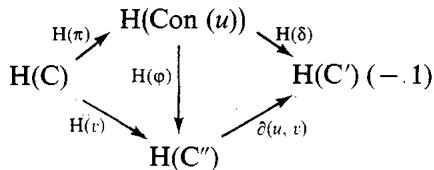
\includegraphics[keepaspectratio]{images/part001_82ee8f27.jpg}}

is commutative and H(φ) is bijective.

In the commutative diagram (10), we have \(\mathrm{H}(1_{\mathbf{C}^{\prime}})\circ \partial (\tilde{u},\tilde{\pi}) = \partial (u,v)\circ \mathrm{H}(\varphi)\) (X, p.~31, prop. 2) and \(\partial (\tilde{u},\tilde{\pi}) = \mathrm{H}(\delta)\) (X, p.~38, lemma 3, b)), hence

\[
\partial (u, v) \circ \mathbf {H} (\varphi) = \mathbf {H} (\delta);
\]

on the other hand, \(\mathrm{H}(v) \circ \mathrm{H}(\beta) = \mathrm{H}(\varphi) \circ \mathrm{H}(\tilde{\pi}) = \mathrm{H}(\varphi) \circ \mathrm{H}(\pi) \circ \mathrm{H}(\beta)\) by X, p.~39, remark. Since \(\mathrm{H}(\beta)\) is bijective, this gives \(\mathrm{H}(v) = \mathrm{H}(\varphi) \circ \mathrm{H}(\pi)\) .

We therefore have \(\partial(u, v) = H(\delta) \circ H(\varphi)^{-1}\) , which provides a new definition of the connecting homomorphism \(\partial(u, v)\) . We also note that if we identify \(H(Con(u))\) with \(H(C'')\) by \(H(\varphi)\) , the preceding corollary means that the exact sequence (8) is then identified with the exact homology sequence relative to (9).

\subsection{Euler-Poincaré characteristics}

In this n°, we consider a set C of classes of A-modules that is additive and left exact, that is, satisfying the following two conditions:

\begin{enumerate}
\def\labelenumi{(\Alph{enumi})}
\item
  If M and N are two A-modules of type C, then M ⊕ N is of type C.
\item
  If \(0 \to \mathbf{M}' \to \mathbf{M} \to \mathbf{M}'' \to 0\) is an exact sequence of A-modules and if \(\mathbf{M}\) and \(\mathbf{M}''\) are of type \(\mathcal{C}\) , then \(\mathbf{M}'\) is of type \(\mathcal{C}\) .
\end{enumerate}

We say that \(\mathcal{C}\) is stable if it satisfies the following conditions, which imply (A) and (G):

\begin{enumerate}
\def\labelenumi{(\Alph{enumi})}
\setcounter{enumi}{4}
\item
  ("C is stable under extensions.") If 0 → M' → M → M'' → 0 is an exact sequence of A-modules and if M' and M'' are of type C, then M is of type C.
\item
  ("C is stable under kernels and cokernels.") For every homomorphism f of A-modules of type C, the A-modules Ker f and Coker f are of type C.
\end{enumerate}

We denote by K( \(\mathcal{C}\) ) the Grothendieck group of \(\mathcal{C}\) and {[}M{]} \(_{\mathcal{C}}\) or {[}M{]} the element of K( \(\mathcal{C}\) ) defined by the A-module M (VIII, § 6, no. 2). Let G be a commutative group and \(\varphi\) a homomorphism from K( \(\mathcal{C}\) ) into G.

Examples. --- 1) If A is a field, one may take for C the set of classes of finite-dimensional vector spaces, and for φ the isomorphism of K(C) onto Z defined by φ({[}M{]}) = dim (M).

\begin{enumerate}
\def\labelenumi{\arabic{enumi})}
\setcounter{enumi}{1}
\tightlist
\item
  One may take for \(\mathcal{C}\) the set of classes of modules of finite length, and for \(\varphi: \mathbf{K}(\mathcal{C}) \to \mathbf{Z}\) the homomorphism defined by \(\varphi([\mathbf{M}]) = \text{long}_{\mathbf{A}}(\mathbf{M})\) .
\end{enumerate}

One says that a graded A-module M is of type C if \(M_{n}\) is of type C for every n (for this, it is necessary, if M is bounded, and sufficient, if C is stable, that the module M be of type C).

DEFINITION 8. --- Let M be a bounded graded A-module of type C and let (M \(_{n}\) ) be its grading. One calls the φ-characteristic of M, and denotes by χφ(M) or simply χ(M), the element ∑ (-1) \(^{n}\) φ({[}M \(_{n}\) {]}) of G.

This definition applies in particular when M is the graded module underlying a complex of A-modules.

Examples. --- 3) If M is bounded of type C, the same is true of M(p) for every \(p \in Z\) , and we have \(\chi(\mathbf{M}(p)) = (-1)^{p} \chi(\mathbf{M})\) .

\begin{enumerate}
\def\labelenumi{\arabic{enumi})}
\setcounter{enumi}{3}
\tightlist
\item
  Let \(0 \to \mathbf{M}' \to \mathbf{M} \to \mathbf{M}'' \to 0\) be an exact sequence of graded A-modules and graded homomorphisms of degree 0. If \(\mathbf{M}, \mathbf{M}'\) and \(\mathbf{M}''\) are bounded of type \(\mathcal{C}\) , we have
\end{enumerate}

\[
\chi (\mathbf {M}) = \chi (\mathbf {M} ^ {\prime}) + \chi (\mathbf {M} ^ {\prime \prime}).
\]

If M and M'' are bounded of type C, the same is true of M'; if C is stable and two of the three modules are bounded of type C, the same is true of the third.

\begin{enumerate}
\def\labelenumi{\arabic{enumi})}
\setcounter{enumi}{4}
\tightlist
\item
  Let \(u: \mathbf{C}' \to \mathbf{C}\) be a morphism of bounded complexes of type \(\mathcal{C}\) . Then Con \((u)\) is bounded of type \(\mathcal{C}\) , and we have:
\end{enumerate}

\[
\chi (\operatorname{Con} (u)) = \chi (\mathbf {C}) - \chi (\mathbf {C} ^ {\prime}).
\]

\begin{enumerate}
\def\labelenumi{\arabic{enumi})}
\setcounter{enumi}{5}
\tightlist
\item
  One can take for G the group K(C) itself, and for φ the identity; we then denote by \(\chi_{\mathcal{C}}(\mathrm{M})\) the element \(\chi_{\varphi}(\mathrm{M}) = \sum (-1)^{n}[\mathrm{M}_{n}]\) of K(C).
\end{enumerate}

Remark. --- One calls the Poincaré polynomial of M relative to \(\varphi\) the element \(\mathrm{P}_{\mathbf{M}}(t) = \sum \varphi([\mathrm{M}_{n}]) t^{n} \in \mathrm{G} \otimes \mathbf{Z}[t, t^{-1}]\) . We have \(\mathrm{P}_{\mathbf{M}}(1) = \varphi([\mathrm{M}])\) and \(\mathrm{P}_{\mathbf{M}}(-1) = \chi(\mathrm{M})\) .

Lemma 4. --- Let C be a bounded complex of type \(\mathcal{C}\) . If H(C) = 0, we have \(\chi(\mathbf{C}) = 0\) . This follows from VIII, § 6, n° 1, cor. of prop. 1.

PROPOSITION 10. --- Let C and C' be two bounded complexes of type C. If there exists a homologism \(u: \mathbf{C}' \to \mathbf{C}\) , we have \(\chi(\mathbf{C}) = \chi(\mathbf{C}')\) .

Indeed, Con \((u)\) is bounded of type \(\mathcal{C}\) and we have \(\chi(\text{Con } (u)) = \chi(\text{C}) - \chi(\text{C}')\) ; on the other hand, H(Con \((u)) = 0\) by X, p.~38, cor., hence \(\chi(\text{Con } (u)) = 0\) (lemma 4).

PROPOSITION 11. --- Let C be a bounded complex of type C.

\begin{enumerate}
\def\labelenumi{\alph{enumi})}
\item
  If \(\mathcal{C}\) is stable, H(C) is of type \(\mathcal{C}\) .
\item
  If H(C) is of type C, then so are B(C) and Z(C), and we have \(\chi(\mathrm{H}(\mathrm{C})) = \chi(\mathrm{C})\) .
\item
  If \(\mathcal{C}\) is stable, for every \(n\) the module \(\mathbf{Z}_n(\mathbf{C})\) is of type \(\mathcal{C}\) as kernel of \(d_n: \mathbf{C}_n \to \mathbf{C}_{n-1}\) , and \(\mathrm{H}_n(\mathbf{C})\) is of type \(\mathcal{C}\) as cokernel of \(\mathbf{C}_{n+1} \to \mathbf{Z}_n\) . On the other hand, \(\mathrm{H}_n(\mathbf{C}) = 0\) as soon as \(\mathbf{C}_n = 0\) .
\item
  Suppose H(C) is of type C. The canonical exact sequences:
\end{enumerate}

\[
0 \to Z _ {n} (\mathbf {C}) \to C _ {n} \to B _ {n - 1} (\mathbf {C}) \to 0
\]

\[
0 \to \mathrm{B} _ {n} (\mathrm{C}) \to \mathrm{Z} _ {n} (\mathrm{C}) \to \mathrm{H} _ {n} (\mathrm{C}) \to 0
\]

show by induction on n starting from the right bound of C that \(Z_{n}(C)\) and \(B_{n}(C)\) are of type C for every n.~We then have

\[
\chi (\mathrm{C}) = \chi (\mathrm{Z} (\mathrm{C})) + \chi (\mathrm{B} (\mathrm{C}) (- 1)) = \chi (\mathrm{Z} (\mathrm{C})) - \chi (\mathrm{B} (\mathrm{C})) = \chi (\mathrm{H} (\mathrm{C})).
\]

COROLLARY. --- If C is stable and C is bounded of type C, the graded module H(C) is bounded of type C and we have \(\chi(\mathrm{H}(\mathrm{C})) = \chi(\mathrm{C})\) .

PROPOSITION 12. --- Let \(0 \to C' \to C \to C'' \to 0\) be an exact sequence of complexes. a) If H(C), H(C') and H(C'') are bounded of type C, we have

\[
\chi (\mathrm{H} (\mathbf {C})) = \chi (\mathrm{H} (\mathbf {C} ^ {\prime})) + \chi (\mathrm{H} (\mathbf {C} ^ {\prime \prime})) .
\]

\begin{enumerate}
\def\labelenumi{\alph{enumi})}
\setcounter{enumi}{1}
\tightlist
\item
  If C is stable, and if two of the graded modules H(C), H(C') and H(C'') are bounded of type C, then so is the third.
\end{enumerate}

Part a) follows from lemma 4 applied to the zero-homology complex defined by the homology exact sequence associated with the given exact sequence. Part b) follows, by considering this homology exact sequence, from the following lemma:

Lemma 5. --- Let M → N → P → Q → R be an exact sequence of A-modules. If C is stable, and if M, N, Q and R are of type C, then the module P is of type C.

Set \(\mathbf{N}' = \operatorname{Coker} (\mathbf{M} \to \mathbf{N})\) and \(\mathbf{Q}' = \operatorname{Ker} (\mathbf{Q} \to \mathbf{R})\) . The modules \(\mathbf{N}'\) and \(\mathbf{Q}'\) are of type \(\mathcal{C}\) , and we have an exact sequence \(0 \to \mathbf{N}' \to \mathbf{P} \to \mathbf{Q}' \to 0\) .

COROLLARY. --- Suppose C is stable, and let \(u : C' \to C\) be a morphism of complexes such that \(\mathrm{H}(\mathbf{C})\) and \(\mathrm{H}(\mathbf{C}')\) are bounded of type C. Then \(\mathrm{H}(\mathrm{Con}(u))\) is bounded of type C, and we have

\[
\chi (\mathrm{H} (\text { Con } (u))) = \chi (\mathrm{H} (\mathrm{C})) - \chi (\mathrm{H} (\mathrm{C} ^ {\prime})) .
\]

This follows from prop. 12 applied to the exact sequence of complexes (X, p.~37, prop. 7)

\[
0 \rightarrow \mathrm{C} \rightarrow \operatorname{Con} (u) \rightarrow \mathrm{C} ^ {\prime} (- 1) \rightarrow 0.
\]

Remark. --- Let E be a complex, \(h: \mathrm{E} \to \mathrm{C}\) and \(h': \mathrm{E} \to \mathrm{C}'\) homotopisms with C and C' bounded of type \(\mathcal{C}\) . We then have \(\chi(\mathrm{C}) = \chi(\mathrm{C}')\) . Indeed, if \(h_1\) is an inverse of \(h\) up to homotopy, \(h' \circ h_1\) is a homotopism, hence a homologism from C to

C' and one can apply prop. 10. Consequently, one can extend definition 8 by setting \(\chi(E) = \chi(C)\) as soon as there exists a homotopism from E to a bounded complex C of type C. Propositions 10, 11, 12 and their corollaries generalize to this setting.

Application:

* Let X be a topological space admitting a finite cell decomposition (cf.~n° 3). a) Let K and K' be two fields, set \(b_i = \dim_K(\mathrm{H}_i(\mathrm{X}, \mathrm{K}))\) and \(b_i' = \dim_K(\mathrm{H}_i(\mathrm{X}, \mathrm{K}'))\) . One does not necessarily have \(b_i = b_i'\) , but one has \(\Sigma(-1)^i b_i = \Sigma(-1)^i b_i'\) .

\begin{enumerate}
\def\labelenumi{\alph{enumi})}
\setcounter{enumi}{1}
\tightlist
\item
  Let \((\mathbf{X}_{n})\) and \((\mathbf{X}_{n}^{\prime})\) be two finite cell decompositions of X, and let \(c_{n}\) and \(c_{n}^{\prime}\) be the number of cells of dimension n in these two decompositions. We have
\end{enumerate}

\[
\Sigma (- 1) ^ {i} c _ {i} = \Sigma (- 1) ^ {i} c _ {i} ^ {\prime}.
\]

\begin{enumerate}
\def\labelenumi{\alph{enumi})}
\setcounter{enumi}{2}
\tightlist
\item
  With the notations of \(a)\) and \(b)\) , we have \(\Sigma(-1)^{i} c_{i} = \Sigma(-1)^{i} b_{i}\) .
\end{enumerate}

The properties \(a\) ) and \(b\) ) follow from \(c\) ), and \(c\) ) follows from prop. 11 applied to the complex \(\Gamma\) described in no. 3, taking for \(\mathscr{C}\) the class of finite-dimensional K-vector spaces and for \(\varphi\) the function defined by \(\varphi([\mathrm{M}]) = \dim_{\mathrm{K}}(\mathrm{M})\) (X, p.~40, example 1). *

\subsection{Complexes of right modules, complexes of multimodules}

A complex of right A-modules is a graded right A-module \((M_{n})_{n\in\mathbf{Z}}\) equipped with a graded endomorphism of degree -1 and square zero; it is therefore a complex of modules over the ring A° opposite to A. All the definitions and properties stated in the preceding sections therefore apply to complexes of right modules considered as complexes of modules over the ring A°.

Similarly, if A and B are two rings, a complex of (A, B)-bimodules is a graded (A, B)-bimodule M equipped with an endomorphism \(d\) graded of degree \((-1)\) and of square zero; if one endows M with its canonical structure of A \(\otimes_{\mathbf{z}} \mathbf{B}^{\circ}\) -module on the left, \(d\) endows it with a structure of A \(\otimes_{\mathbf{z}} \mathbf{B}^{\circ}\) -complex. All definitions and properties stated in the preceding sections therefore apply to complexes of bimodules. Complexes of multimodules are defined analogously.

\subsection{Example: de Rham complex}

In this section, we assume that A is a commutative \(k\) -algebra over a commutative ring \(k\) . One denotes by \(\Omega_{\mathbf{A}/k}^{1}\) the A-module of Kähler differentials of A (III, p.~134), \(d^{0}: \mathbf{A} \to \Omega_{\mathbf{A}/k}^{1}\) the \(k\) -derivation \(d_{\mathbf{A}/k}\) , and \(\Omega_{\mathbf{A}/k}\) the graded \(k\) -algebra \(\boldsymbol{\Lambda}_{\mathbf{A}}(\Omega_{\mathbf{A}/k}^{1})\) .

PROPOSITION 13. — There exists a unique k-antiderivation \(d: \Omega_{\mathbf{A}/k} \to \Omega_{\mathbf{A}/k}\) of degree 1, with square zero, extending the derivation \(d^{0}: \mathbf{A} \to \Omega_{\mathbf{A}/k}^{1}\) .

Let us prove the uniqueness of the antiderivation \(d\) . Since \(d \circ d = 0\) we have, for \(y, x_1, \ldots, x_p \in \mathbf{A}\) :

\[
d \left(y d x _ {1} \wedge \dots \wedge d x _ {p}\right) = d y \wedge d x _ {1} \wedge \dots \wedge d x _ {p}.
\]

The A-module \(\Omega_{\mathbf{A}/k}^{p}\) being generated by the elements \(dx_{1} \wedge \ldots \wedge dx_{p}\) , this proves the uniqueness of \(d\) .

To prove existence, it suffices to construct a \(k\) -homomorphism \(d^{1}:\Omega_{\mathbb{A}/k}^{1}\to\Omega_{\mathbb{A}/k}^{2}\) such that \(d^{1}\circ d^{0}=0\) and

\[
d ^ {1} (a \omega) = d ^ {0} (a) \wedge \omega + a d ^ {1} (\omega) \quad \text {for} \quad a \in A, \quad \omega \in \Omega_ {A k} ^ {1}.\tag{11}
\]

Indeed, it then follows from III, p.~128, prop. 14 (taking into account III, p.~118, remark 2) that there exists an antiderivation \(d: \Omega_{\mathbf{A}/k} \to \Omega_{\mathbf{A}/k}\) that coincides with \(d^{0}\) in degree 0 and with \(d^{1}\) in degree 1. Since \(d^{0}\) vanishes on \(\mathbf{A}\) , the antiderivation \(d\) is \(k\) -linear; since \(d^{1} \circ d^{0} = 0\) , we have \(d \circ d = 0\) since \(\Omega_{\mathbf{A}/k}\) is generated as \(\mathbf{A}\) -algebra by the elements \(d^{0} a\) for \(a \in \mathbf{A}\) .

To define \(d^{1}\) , recall (III, p. 133) that \(\Omega_{\mathbf{A}/k}^{1}\) is equal to the A-module \(\mathfrak{I}/\mathfrak{I}^{2}\) , where \(\mathfrak{I}\) is the kernel of the multiplication \(m: \mathbf{A} \otimes_{k} \mathbf{A} \to \mathbf{A}\) . Consider the \(k\) -linear map \(u: \mathbf{A} \otimes_{k} \mathbf{A} \to \Omega_{\mathbf{A}/k}^{2}\) defined by \(u(x \otimes y) = d^{0}(y) \wedge d^{0}(x)\) . We have

\[
u (a x \otimes y - x \otimes a y) = d ^ {0} (y) \wedge d ^ {0} (a x) - d ^ {0} (a y) \wedge d ^ {0} (x) = d ^ {0} (x y) \wedge d ^ {0} (a)
\]

for x, y, and a in A, whence

\[
u ((a \otimes 1 - 1 \otimes a) \xi) = d ^ {0} (m (\xi)) \wedge d ^ {0} (a), \quad \xi \in \mathrm{A} \otimes_ {k} \mathrm{A}, \quad a \in \mathrm{A}. \tag {12}
\]

Since \(\mathfrak{I}\) is generated as a left A-module by the elements ( \(a \otimes 1 - 1 \otimes a\) ) for \(a \in \mathbf{A}\) , we deduce that \(u(\mathfrak{I}^2) = 0\) ; therefore \(u\) defines by restriction to \(\mathfrak{I}\) and passage to the quotient a \(k\) -linear map \(d^1: \mathfrak{I}/\mathfrak{I}^2 \to \Omega_{\mathrm{A}/k}^2\) .

By making \(\xi = b \otimes 1\) in (12), with \(b \in \mathbf{A}\) , we obtain \(d^{1}(bd^{0}(a)) = d^{0}(b) \wedge d^{0}(a)\) ; it follows that \(d^{1} \circ d^{0} = 0\) and that \(d^{1}(c\omega) = d^{0}(c) \wedge \omega + cd^{1}(\omega)\) for \(c \in \mathbf{A}\) and \(\omega = bd^{0}(a)\) . Since \(\Omega_{\mathbf{A}/k}^{1}\) is generated as \(k\) -module by the elements \(bd^{0}(a)\) , for \(a\) and \(b\) in \(\mathbf{A}\) , formula (11) is satisfied for all \(\omega \in \Omega_{\mathbf{A}/k}\) , which completes the proof of the proposition.

Sometimes it is said that the elements \(\omega\in\Omega_{A/k}^{p}\) are the exterior differential forms of degree \(p\) of A over \(k\) and that the antiderivation \(d\) is the exterior differential of \(\Omega_{A/k}\) ; the complex ( \(\Omega_{A/k}\) , \(d\) ) is called the de Rham complex of A over \(k\) , and its homology is the de Rham cohomology of A over \(k\) .

Example 1. --- Take for A the ring \(k[\mathbf{X}_{1},\ldots,\mathbf{X}_{n}]\) . Then \(\Omega_{\mathbf{A}/k}^{1}\) is a free A-module with basis \(d\mathbf{X}_{1},\ldots,d\mathbf{X}_{n}\) (III, p.~134, example). Consequently, if for every subset \(\mathrm{I}=\{i_{1},\ldots,i_{p}\}\) of \([1,n]\) we set \(d\mathbf{X}_{\mathrm{I}}=d\mathbf{X}_{i_{1}}\wedge\ldots\wedge d\mathbf{X}_{i_{p}}\) (with \(i_{1}<\ldots<i_{p}\) ), the A-module \(\Omega_{\mathbf{A}/k}^{p}\) admits as a basis the elements \(d\mathbf{X}_{\mathrm{I}}\) , where I ranges over the set of subsets of \([1,n]\) of cardinality \(p\) . We have

\[
d (\mathrm{P} d \mathrm{X} _ {\mathrm{I}}) = d \mathrm{P} \wedge d \mathrm{X} _ {\mathrm{I}} = \sum_ {i \notin \mathrm{I}} (- 1) ^ {n (\mathrm{I}, i)} \frac {\partial \mathrm{P}}{\partial \mathrm{X} _ {i}} d \mathrm{X} _ {\mathrm{I} \cup \{i \}},
\]

where \(n(\mathbf{I}, i)\) denotes the number of elements of I strictly less than \(i\) .

The cycles of \(Z^{p}(\Omega_{\mathbf{A}/k})\) are therefore the elements \(\omega = \sum_{\text{Card (I)} = p} \mathrm{P}_{\mathrm{I}} d\mathrm{X}_{\mathrm{I}}\) such that, for every subset \(J\) with \((p + 1)\) elements of \([1, n]\) , one has:

\[
\sum_ {i \in J} (- 1) ^ {n (J, i)} \frac {\partial P _ {J - \{i \}}}{\partial X _ {i}} = 0.
\]

The element ω is a boundary if one can choose, for every subset \(J \subset [1, n]\) with \((p - 1)\) elements, a polynomial \(Q_{J} \in A\) such that:

\[
\mathrm{P} _ {\mathrm{I}} = \sum_ {j \in \mathrm{I}} (- 1) ^ {n (\mathrm{I}, j)} \frac {\partial \mathrm{Q} _ {\mathrm{I} - \{j \}}}{\partial \mathrm{X} _ {j}}.
\]

We will see in § 9 that the de Rham complex of A over k is acyclic in degrees \textgreater{} 0 if k is a Q-algebra (X, p.~159, remark 4).

* Example 2. --- Suppose that \(k = \mathbf{C}\) and \(\mathbf{A} = \mathbf{C}\) \([\mathrm{X}_1, \ldots, \mathrm{X}_n] / (\mathrm{P}_1, \ldots, \mathrm{P}_r)\) , where the \(\mathrm{P}_i\) are polynomials in \(\mathrm{X}_1, \ldots, \mathrm{X}_n\) , such that the set of points of \(\mathbf{C}^n\) where all the \(\mathrm{P}_i\) vanish is an analytic submanifold V of \(\mathbf{C}^n\) . One can show that the de Rham cohomology of A over C is isomorphic to the singular cohomology H(V, C). *

Let M be an A-module and \(\nabla^{0}\) a \(k\) -linear map from M into \(\mathbf{M} \otimes_{\mathbf{A}} \Omega_{\mathbf{A}/k}^{1}\) such that

\[
\nabla^ {0} (a m) = a \nabla^ {0} (m) + m \otimes d a \quad \text { for } \quad a \in \mathrm{A}, \quad m \in \mathrm{M}\tag{13}
\]

(one sometimes says that \(\nabla^{0}\) is a connection on the A-module M).

Proposition 14. --- (i) There exists a unique k-linear map \(\nabla\) of the \(\Omega_{\mathbf{A}/k}\) right module \(\mathbf{M} \otimes_{\mathbf{A}} \Omega_{\mathbf{A}/k}\) into itself, graded of degree 1, which extends \(\nabla^{0}\) in degree 0 and satisfies the identity:

\[
\nabla (x \omega) = (\nabla x) \omega + (- 1) ^ {p} x (d \omega) \quad \mathrm{for} \quad x \in \mathrm{M} \otimes_ {\mathrm{A}} \Omega_ {\mathrm{A} / k} ^ {p}, \quad \omega \in \Omega_ {\mathrm{A} / k}. \tag {14}
\]

\begin{enumerate}
\def\labelenumi{(\roman{enumi})}
\setcounter{enumi}{1}
\tightlist
\item
  The composite mapping \(\nabla \circ \nabla\) is \(\Omega_{\mathbf{A} / k}\) -linear; in particular the map \(\mathbf{R} = \nabla^{1} \circ \nabla^{0}\) of \(\mathbf{M}\) to \(\mathbf{M} \otimes_{\mathbf{A}} \Omega_{\mathbf{A} / k}^{2}\) is \(\mathbf{A}\) -linear, and we have
\end{enumerate}

\[
\nabla \circ \nabla (m \otimes \omega) = R (m). \omega \quad \mathrm{for} \quad m \in M, \quad \omega \in \Omega_ {A / k}.
\]

The homomorphism R is sometimes called the curvature homomorphism of the connection \(\nabla^{0}\) ; if it is zero, the pair \((\mathbf{M} \otimes_{\mathbf{A}} \Omega_{\mathbf{A}/k}, \nabla)\) is a complex, also called the de Rham complex of \((\mathbf{M}, \nabla^{0})\) over \(k\) .

Let us prove (i). The uniqueness of \(\nabla\) is obvious. Let us define a \(k\) -homomorphism \(\overline{\nabla}\) of \(\mathbf{M} \otimes_k \Omega_{\mathbf{A}/k}\) to \(\mathbf{M} \otimes_{\mathbf{A}} \Omega_{\mathbf{A}/k}\) by

\[
\overline {{{\nabla}}} (m \otimes_ {k} \omega) = (\nabla^ {0} m) \omega + m \otimes d \omega \quad \text { for } \quad m \in \mathbf {M}, \quad \omega \in \Omega_ {\mathrm{A} / k}.
\]

It follows from (13) that \(\overline{\nabla}(am \otimes \omega) = \overline{\nabla}(m \otimes a\omega)\) , so that by passing to the quotient we obtain a \(k\) -homomorphism \(\nabla\) of \(\mathbf{M} \otimes_{\mathbf{A}} \Omega_{\mathbf{A}/k}\) into itself, graded of degree 1, extending \(\nabla^{0}\) in degree 0. Let us verify (14): we have, for \(m \in \mathbf{M}\) , \(\alpha \in \Omega_{\mathbf{A}/k}^{p}\) , \(\omega \in \Omega_{\mathbf{A}/k}\) :

\[
\begin{array}{r l} \nabla ((m \otimes \alpha). \omega) & = \nabla (m \otimes (\alpha \wedge \omega)) = \nabla^ {0} (m). (\alpha \wedge \omega) + m \otimes d (\alpha \wedge \omega) \\ & = \nabla^ {0} (m) \alpha . \omega + (m \otimes d \alpha) \omega + (- 1) ^ {p} (m \otimes \alpha) d \omega \\ & = (\nabla (m \otimes \alpha)) \omega + (- 1) ^ {p} (m \otimes \alpha) d \omega \end{array}
\]

which proves (14) for \(x = m \otimes \alpha\) ; the general case follows from this by linearity.

Let us prove (ii). Let \(x \in \mathbf{M} \otimes_{\mathbf{A}} \Omega_{\mathbf{A}/k}^{p}\) , \(\omega \in \Omega_{\mathbf{A}/k}\) ; by repeated application of (14), we obtain:

\[
\begin{array}{r l} \nabla \circ \nabla (x \omega) = & \nabla (\nabla (x) \omega) + (- 1) ^ {p} \nabla (x d \omega) \\ & = (\nabla \circ \nabla (x)) \omega + (- 1) ^ {p + 1} \nabla (x) (d \omega) + (- 1) ^ {p} \nabla (x) (d \omega) \\ & = (\nabla \circ \nabla (x)) \omega , \end{array}
\]

which proves the first assertion of (ii); the others follow immediately.

\section{RESOLUTIONS}

We keep the conventions of the preceding paragraph.

\subsection{Extension of morphisms of complexes}

Lemma 1. --- Consider a diagram of A-modules and homomorphisms

\[
\begin{array}{c} \mathbf {M} ^ {\prime} \xrightarrow {\alpha^ {\prime}} \mathbf {M} \xrightarrow {\alpha} \mathbf {M} ^ {\prime \prime} \\ f ^ {\prime} \Biggl \downarrow \quad \swarrow k / f \Biggl \downarrow \quad \swarrow k ^ {\prime \prime} \\ \mathbf {N} ^ {\prime} \xrightarrow [ \beta^ {\prime} ]{} \mathbf {N} \xrightarrow [ \beta ]{} \mathbf {N} ^ {\prime \prime} \end{array}
\]

such that \(f \circ \alpha' = \beta \circ f', \alpha \circ \alpha' = 0\) , Ker \(\beta = \operatorname{Im} \beta'\) , and \(f = k'' \circ \alpha + \beta \circ k\) and where \(\mathbf{M}'\) is projective. There exists an A-homomorphism \(k': \mathbf{M}' \to \mathbf{N}'\) such that \(f' = k \circ \alpha' + \beta' \circ k'\) .

Indeed, set \(g = f' - k \circ \alpha'\) ; we have

\[
\beta \circ g = \beta \circ f ^ {\prime} - \beta \circ k \circ \alpha^ {\prime} = f \circ \alpha^ {\prime} - \beta \circ k \circ \alpha^ {\prime} = k ^ {\prime \prime} \circ \alpha \circ \alpha^ {\prime} = 0.
\]

This implies \(\operatorname{Im}(g) \subset \operatorname{Ker}(\beta) = \operatorname{Im}(\beta')\) . Since \(\mathbf{M}'\) is projective, there therefore exists an A-homomorphism \(k': \mathbf{M}' \to \mathbf{N}'\) such that \(\beta' \circ k' = g\) , whence the lemma.

Lemma 2. --- If in the commutative diagram of A-modules and homomorphisms

\[
\begin{array}{c c c c c} \mathbf {M} ^ {\prime} & \xrightarrow {\alpha^ {\prime}} & \mathbf {M} & \xrightarrow {\alpha} & \mathbf {M} ^ {\prime \prime} \\ & & \Big \downarrow^ {u} & & \Big \downarrow^ {u ^ {\prime \prime}} \\ \mathbf {N} ^ {\prime} & \xrightarrow {\beta^ {\prime}} & \mathbf {N} & \xrightarrow {\beta} & \mathbf {N} ^ {\prime \prime} \end{array}
\]

we have \(\alpha\circ\alpha'\) =0, Ker \(\beta=\operatorname{Im}\beta'\) and if \(\mathbf{M}'\) is projective, there exists an A-homomorphism \(u':\mathbf{M}'\to\mathbf{N}'\) such that \(\beta'\circ u'=u\circ\alpha'\) .

It suffices to set \(k'' = u'', k = -u, f = 0, f' = 0\) and \(u' = k'\) in Lemma 1.

Lemma 1 bis. --- Consider a diagram of A-modules and homomorphisms

\[
\begin{array}{c} \mathbf {M} ^ {\prime} \xrightarrow {\alpha^ {\prime}} \mathbf {M} \xrightarrow {\alpha} \mathbf {M} ^ {\prime \prime} \\ \Big \downarrow_ {k ^ {\prime}} \Big \downarrow_ {f ^ {\prime}} \Big \downarrow_ {k} \Big \downarrow_ {f} \\ \mathbf {N} ^ {\prime} \xrightarrow [ \beta^ {\prime} ]{} \mathbf {N} \xrightarrow [ \beta ]{} \mathbf {N} ^ {\prime \prime} \end{array}
\]

such that \(f \circ \alpha' = \beta \circ f'\) , Ker \(\alpha = \operatorname{Im} \alpha'\) , \(\beta \circ \beta' = 0\) , and \(f' = k \circ \alpha' + \beta' \circ k'\) and where \(N''\) is injective. There exists an A-homomorphism \(k'' : M'' \to N''\) such that \(f = k'' \circ \alpha + \beta \circ k\) . Indeed, set \(q = f - \beta \circ k\) , we have

\[
g \circ \alpha^ {\prime} = f \circ \alpha^ {\prime} - \beta \circ k \circ \alpha^ {\prime} = \beta \circ f ^ {\prime} - \beta \circ k \circ \alpha^ {\prime} = \beta \circ \beta^ {\prime} \circ k ^ {\prime} = 0.
\]

This implies Ker \(g \supset \operatorname{Im} \alpha' = \operatorname{Ker} \alpha\) . Since \(\mathbf{N}''\) is injective, there therefore exists (X, p.~16, remark) an A-homomorphism \(k': \mathbf{M}'' \to \mathbf{N}''\) such that \(g = k'' \circ \alpha\) , whence the lemma.

Lemma 2 bis. --- If, in the commutative diagram of A-modules and homomorphisms

\[
\begin{array}{c c c c c} \mathbf {M} ^ {\prime} & \stackrel {{\alpha^ {\prime}}} {{\longrightarrow}} & \mathbf {M} & \stackrel {{\alpha}} {{\longrightarrow}} & \mathbf {M} ^ {\prime \prime} \\ u ^ {\prime} \Big \downarrow & & u \Big \downarrow & & \\ \mathbf {N} ^ {\prime} & \stackrel {{\beta^ {\prime}}} {{\longrightarrow}} & \mathbf {N} & \stackrel {{\beta}} {{\longrightarrow}} & \mathbf {N} ^ {\prime \prime}, \end{array}
\]

we have \(\operatorname{Ker} \alpha = \operatorname{Im} \alpha'\) , \(\beta \circ \beta' = 0\) and if \(\mathbf{N}''\) is injective, there exists an A-homomorphism \(u'' : \mathbf{M}'' \to \mathbf{N}''\) such that \(u'' \circ \alpha = \beta \circ u\) .

It suffices to set \(u' = k', u = -k, f = 0, f' = 0\) and \(k'' = u''\) in Lemma 1 bis.

PROPOSITION 1. --- Let (P, \(d_{\mathbb{P}}\) ) and (E, \(d_{\mathbb{E}}\) ) be two complexes of A-modules and r an integer.

\begin{enumerate}
\def\labelenumi{\alph{enumi})}
\item
  Let \((u_i: \mathrm{P}_i \to \mathrm{E}_i)_{i \leqslant r}\) be a family of homomorphisms such that \(d_{\mathrm{E}} \circ u_i = u_{i-1} \circ d_P\) for \(i \leqslant r\) . Suppose that \(\mathrm{P}_i\) is projective for \(i > r\) and that \(\mathrm{H}_i(\mathrm{E}) = 0\) for \(i \geqslant r\) . Then the family of the \(u_i\) extends to a morphism of complexes from P to E; two such extensions are homotopic.
\item
  Let \((u^{i}:\mathbf{P}^{i}\to\mathbf{E}^{i})_{i\leqslant r}\) be a family of homomorphisms such that \(u^{i}\circ d_{\mathrm{P}}=d_{\mathrm{E}}\circ u^{i-1}\) for \(i\leqslant r\) . Suppose that \(\mathbf{E}^{i}\) is injective for \(i>r\) and that \(\mathbf{H}^{i}(\mathbf{P})=0\) for \(i\geqslant r\) . Then the family of the \(u^{i}\) extends to a morphism of complexes from \(\mathbf{P}\) to \(\mathbf{E}\) ; two such extensions are homotopic.
\end{enumerate}

Let us prove a). The existence of an extension v of the family \((u_{i})_{i\leqslant r}\) follows immediately from Lemma 2 by induction. Let \(v'\) be another extension; set \(f=v'-v\) , and construct by induction on the integer n a homomorphism \(k_{n}:P_{n}\to E_{n+1}\) such that \(f_{n}=d_{E}\circ k_{n}+k_{n-1}\circ d_{P}\) . For \(i\leqslant r\) , take \(k_{i}=0\) . Let \(n\geqslant r\) and suppose the \(k_{i}\) constructed for \(i\leqslant n\) . Consider then the diagram

\[
\begin{array}{c} \mathrm{P} _ {n + 1} \xrightarrow {d _ {\mathrm{p}}} \mathrm{P} _ {n} \xrightarrow {d _ {\mathrm{p}}} \mathrm{P} _ {n - 1} \\ f _ {n + 1} \Biggl \downarrow \quad k _ {n} \Biggl \downarrow f _ {n} \Biggl \downarrow k _ {n - 1} \\ \mathrm{E} _ {n + 2} \xrightarrow {d _ {\mathrm{E}}} \mathrm{E} _ {n + 1} \xrightarrow {d _ {\mathrm{E}}} \mathrm{E} _ {n}. \end{array}
\]

The hypotheses of Lemma 1 are satisfied; there therefore exists an A-homomorphism \(k_{n+1}: \mathbf{P}_{n+1} \to \mathbf{E}_{n+2}\) such that \(f_{n+1} = d_{\mathbf{E}} \circ k_{n+1} + k_n \circ d_p\) , whence \(a\) ).

The proof of b) is analogous, via Lemmas 1 bis and 2 bis.

\subsection{Resolutions}

In what follows, one always identifies a module with the complex of which it is the degree-zero component and of which all other components are zero.

DEFINITION 1. --- Let M be an A-module. A left resolution of M is a pair (P, p) where P is a complex zero to the right and p : P → M is a homologism. A right resolution of M is a pair (e, E) where E is a complex zero to the left and e : M → E a homologism.

One calls the length of the resolution (P, p) (resp. (e, E)) the length of the complex P (resp. E). If (P, p) and (P', p') (resp. (e, E) and (e', E')) are two left (resp. right) resolutions of M, a morphism of complexes \(f: P \to P'\) such that \(p' \circ f = p\) (resp. \(g: E \to E'\) such that \(g \circ e = e'\) ) is called a morphism of resolutions.

PROPOSITION 2. --- Let P be a complex that is zero on the right and let p : P → M be a morphism. For (P, p) to be a left resolution of M, it is necessary and sufficient that the sequence

\[
\dots \longrightarrow \mathrm{P} _ {n} \xrightarrow {d _ {\mathrm{P}}} \mathrm{P} _ {n - 1} \longrightarrow \dots \quad \longrightarrow \mathrm{P} _ {1} \xrightarrow {d _ {\mathrm{P}}} \mathrm{P} _ {0} \xrightarrow {p _ {0}} \mathrm{M} \longrightarrow 0\tag{1}
\]

be exact.

Indeed, to say that \(p: \mathbf{P} \to \mathbf{M}\) is a homologism means that \(\mathrm{H}_{i}(\mathbf{P}) = 0\) for \(i > 0\) and that \(p_{0}\) induces an isomorphism from Coker ( \(d_{\mathbf{P}}: \mathbf{P}_{1} \to \mathbf{P}_{0}\) ) onto \(\mathbf{M}\) .

Similarly:

PROPOSITION 2bis. --- Let E be a complex that is zero on the left and let e : M → E be a morphism. For (e, E) to be a right resolution of M, it is necessary and sufficient that the sequence

\[
0 \longrightarrow \mathrm{M} \stackrel {e _ {0}} {\longrightarrow} \mathrm{E} ^ {0} \stackrel {d _ {\mathrm{E}}} {\longrightarrow} \mathrm{E} ^ {1} \longrightarrow \dots \longrightarrow \mathrm{E} ^ {n} \stackrel {d _ {\mathrm{E}}} {\longrightarrow} \mathrm{E} ^ {n + 1} \longrightarrow \dots\tag{1 bis}
\]

be exact.

By abuse of language, one often says that the sequence (1) (resp. (1 bis)) is a left (resp. right) resolution of M.

DEFINITION 2. --- A projective (resp. free, resp. flat) resolution of the A-module M is a left resolution (P, p) of M such that the complex P is projective (resp. free, resp. flat) (X, p.~25). An injective resolution of M is a right resolution (e, E) of M such that the complex E is injective (loc. cit.).

Examples. --- 1) Suppose that the ring A is principal; let M be an A-module and \((x_{i})_{i\in I}\) a generating family of M. Let \(L_{0}\) be the free module \(\mathbf{A}^{(I)}\) , \((e_{i})\) its canonical basis, and define \(p:L_{0}\to\mathbf{M}\) by \(p(e_{i})=x_{i}\) . The morphism \(p\) is surjective and its kernel \(L_{1}\) is a free A-module by VII, § 3, cor. 2 to th. 1, so the exact sequence

\[
0 \to \mathrm{L} _ {1} \to \mathrm{L} _ {0} \xrightarrow {p} \mathrm{M} \to 0
\]

is a free resolution of M of length 1. If I is finite, \(L_{0}\) and \(L_{1}\) are finitely generated.

\begin{enumerate}
\def\labelenumi{\arabic{enumi})}
\setcounter{enumi}{1}
\tightlist
\item
  Suppose A is commutative; let E be an A-module and u an endomorphism of E. Denote by \(E_{u}\) the A{[}X{]}-module obtained by endowing E with the structure defined by
\end{enumerate}

\[
(p, x) \mapsto p (u) (x) \quad \text { for } \quad p \in \mathrm{A} [ \mathrm{X} ] \quad \text { and } \quad x \in \mathrm{E}.
\]

By III, p.~106, we have an exact sequence:

\[
0 \to \mathrm{A} [ \mathrm{X} ] \otimes_ {\mathrm{A}} \mathrm{E} \stackrel {\psi} {\to} \mathrm{A} [ \mathrm{X} ] \otimes_ {\mathrm{A}} \mathrm{E} \stackrel {\varphi} {\to} \mathrm{E} _ {u} \to 0
\]

where \(\varphi(p \otimes x) = p.x\) and \(\psi(p \otimes x) = Xp \otimes x - p \otimes u(x)\) for \(p \in A[X]\) and \(x \in E\) . This exact sequence is a resolution of length 1 of \(E_u\) free (resp. projective, resp. finitely generated) if E is a free (resp. projective, resp. finitely generated) A-module. 3) If A is principal, the exact sequence

\[
0 \rightarrow \mathrm{A} \rightarrow \mathrm{K} \rightarrow \mathrm{K/A} \rightarrow 0
\]

is an injective resolution of length 1 of the A-module \(\mathbf{A}_s\) (X, p.~18, example 1).

PROPOSITION 3. — Let \(f: \mathbf{M}' \to \mathbf{M}\) be a homomorphism of A-modules, \(p': \mathbf{P}' \to \mathbf{M}'\) be a morphism into \(\mathbf{M}'\) of a complex that is zero on the right and projective \(\mathbf{P}'\) , and \(p: \mathbf{P} \to \mathbf{M}\) a left resolution of M. There exists a morphism of complexes \(\tilde{f}: \mathbf{P}' \to \mathbf{P}\) and one only up to homotopy, such that \(p \circ \tilde{f} = f \circ p'\) .

Consider the complex \(\overline{\mathbf{P}}\) defined as follows: \(\overline{\mathbf{P}}_n = \mathbf{P}_n\) for \(n \neq -1\) , \(\overline{\mathbf{P}}_{-1} = \mathbf{M}\) , \(d_{\overline{\mathbf{P}},n} = d_{\mathbf{P},n}\) for \(n \neq 0, -1\) , \(d_{\overline{\mathbf{P}},0} = p_0\) , \(d_{\overline{\mathbf{P}},-1} = 0\) , and the complex \(\overline{\mathbf{P}}'\) defined analogously. Applying to the complexes \(\overline{\mathbf{P}}\) and \(\overline{\mathbf{P}}'\) prop. 1 a) with \(r=0\) , \(u_i = 0\) for \(i < -1\) and \(u_{-1} = f\) , we obtain prop. 3.

COROLLARY. — Let (P, p) and (P', p') be two projective resolutions of M. There exists one and only one homotopism up to homotopy \(\alpha: P' \to P\) such that \(p \circ \alpha = p'\) .

Indeed, there exists a morphism \(\alpha: P' \to P\) (resp. \(\beta: P \to P'\) ) such that \(p \circ \alpha = p'\) (resp. \(p' \circ \beta = p\) ). Since \(p \circ \alpha \circ \beta = p\) (resp. \(p' \circ \beta \circ \alpha = p'\) ), \(\alpha \circ \beta\) is homotopic to \(1_P\) (resp. \(\beta \circ \alpha\) is homotopic to \(1_{P'}\) ).

PROPOSITION 3 bis. — Let \(g: \mathbf{N} \to \mathbf{N}'\) be a homomorphism of A-modules, \(e': \mathbf{N}' \to \mathbf{E}'\) a morphism of \(\mathbf{N}'\) into a complex that is zero on the left and injective \(\mathbf{E}'\) , and \(e: \mathbf{N} \to \mathbf{E}\) a right resolution of \(\mathbf{N}\) . There exists a morphism of complexes \(\tilde{g}: \mathbf{E} \to \mathbf{E}'\) and one only up to homotopy, such that \(\tilde{g} \circ e = e' \circ g\) .

This is proved like Prop. 3 with the aid of Prop. 1 b).

COROLLARY. --- Let \((e, E)\) and \((e', E')\) be two injective resolutions of N; there exists a homotopism \(\alpha : E \to E'\) and only one up to homotopy such that \(\alpha \circ e = e'\) .

\subsection{The canonical free resolution}

For every A-module M, denote by \(\mathbf{L}_{0}(\mathbf{M})\) the free A-module \(\mathbf{A}^{(\mathbf{M})}\) with basis M, \((e_{m})_{m\in\mathbf{M}}\) its canonical basis and \(p_{\mathbf{M}}:\mathbf{L}_{0}(\mathbf{M})\to\mathbf{M}\) the homomorphism such that

\[
p _ {\mathbf {M}} (e _ {m}) = m, \quad m \in \mathbf {M}.
\]

Set \(Z_0(\mathbf{M}) = \operatorname{Ker} p_{\mathbf{M}}\) and let \(i_{\mathbf{M}}: Z_0(\mathbf{M}) \to L_0(\mathbf{M})\) be the canonical injection. We have an exact sequence

\[
0 \longrightarrow Z _ {0} (\mathrm{M}) \stackrel {i _ {\mathrm{M}}} {\longrightarrow} L _ {0} (\mathrm{M}) \stackrel {p _ {\mathrm{M}}} {\longrightarrow} \mathrm{M} \longrightarrow 0.\tag{1}
\]

We define a graded module L(M) by setting \(\mathrm{L}_{n}(\mathrm{M}) = 0\) for n \textless{} 0 and, by induction on the integer n \textgreater{} 0

\[
\mathrm{L} _ {n} (\mathrm{M}) = \mathrm{L} _ {0} \left(\mathrm{Z} _ {n - 1} (\mathrm{M})\right); \quad \mathrm{Z} _ {n} (\mathrm{M}) = \mathrm{Z} _ {0} \left(\mathrm{Z} _ {n - 1} (\mathrm{M})\right).\tag{2}
\]

We define A-homomorphisms \(d_{n}^{\mathbf{M}}:\mathrm{L}_{n}(\mathbf{M})\to \mathrm{L}_{n - 1}(\mathbf{M})\) by

\[
\left\{ \begin{array}{l l} d _ {n} ^ {\mathbf {M}} = 0, & n \leqslant 0, \\ d _ {1} ^ {\mathbf {M}} = i _ {\mathbf {M}} \circ p _ {\mathbf {Z} _ {0} (\mathbf {M})}, & \\ d _ {n} ^ {\mathbf {M}} = i _ {\mathbf {Z} _ {n - 2} (\mathbf {M})} \circ p _ {\mathbf {Z} _ {n - 1} (\mathbf {M})}, & n > 1. \end{array} \right.\tag{3}
\]

By construction, we have an exact sequence

\[
\longrightarrow \mathrm{L} _ {n} (\mathrm{M}) \xrightarrow {d _ {n} ^ {\mathrm{M}}} \mathrm{L} _ {n - 1} (\mathrm{M}) \longrightarrow \dots \longrightarrow \mathrm{L} _ {0} (\mathrm{M}) \xrightarrow {p _ {\mathrm{M}}} \mathrm{M} \longrightarrow 0,
\]

so that, if one extends \(p_{\mathbf{M}}\) as a morphism of complexes

\[
p _ {\mathbf {M}}: (\mathrm{L} (\mathbf {M}), d ^ {\mathbf {M}}) \rightarrow \mathbf {M},
\]

one obtains a free resolution of M, called the canonical free resolution of M.

Let \(f: \mathbf{M} \to \mathbf{N}\) be a homomorphism of A-modules. Denote by

\[
\mathrm{L} _ {0} (f): \mathrm{L} _ {0} (\mathrm{M}) \rightarrow \mathrm{L} _ {0} (\mathrm{N})
\]

the unique A-homomorphism such that \(L_0(f)(e_m) = e_{f(m)}\) for all \(m \in \mathbf{M}\) . We have

\[
p _ {\mathbf {N}} \circ \mathrm{L} _ {0} (f) = f \circ p _ {\mathbf {M}}.\tag{4}
\]

Consequently, \(L_0(f)\) induces an A-homomorphism \(Z_0(f):Z_0(M)\to Z_0(N)\) and we have

\[
i _ {\mathbf {N}} \circ \mathbf {Z} _ {0} (f) = \mathbf {L} _ {0} (f) \circ i _ {\mathbf {M}}.\tag{5}
\]

Set \(\mathrm{L}_{n}(f)=0\) , for n\textless0 and define by induction on the integer n\textgreater0, homomorphisms \(\mathrm{L}_{n}(f):\mathrm{L}_{n}(\mathrm{M})\to\mathrm{L}_{n}(\mathrm{N})\) and \(\mathrm{Z}_{n}(f):\mathrm{Z}_{n}(\mathrm{M})\to\mathrm{Z}_{n}(\mathrm{N})\) by

\[
\left\{ \begin{array}{l} \mathrm{L} _ {n} (f) = \mathrm{L} _ {0} (\mathrm{Z} _ {n - 1} (f)) \\ \mathrm{Z} _ {n} (f) = \mathrm{Z} _ {0} (\mathrm{Z} _ {n - 1} (f)). \end{array} \right.\tag{6}
\]

PROPOSITION 4. --- L(f) : L(M) → L(N) is a morphism of complexes of A-modules; moreover, we have \(p_{\mathbf{M}} \circ \mathrm{L}(f) = f \circ p_{\mathbf{N}}\) .

We need to prove that, for every integer n \textgreater{} 0 , the formula

\[
d _ {n} ^ {\mathbf {N}} \circ \mathrm{L} _ {n} (f) = \mathrm{L} _ {n - 1} (f) \circ d _ {n} ^ {\mathbf {M}}.
\]

We first have

\[
\begin{array}{r l r l} d _ {1} ^ {\mathbf {N}} \circ \mathrm{L} _ {1} (f) & = i _ {\mathrm{N}} \circ p _ {\mathbf {Z} _ {0} (\mathbf {N})} \circ \mathrm{L} _ {0} (\mathbf {Z} _ {0} (f)) & & (\mathrm {by~(3)~and~(6)}) \\ & = i _ {\mathrm{N}} \circ \mathrm{Z} _ {0} (f) \circ p _ {\mathbf {Z} _ {0} (\mathbf {M})} & & (\mathrm {by~(4)}) \\ & = \mathrm{L} _ {0} (f) \circ i _ {\mathbf {M}} \circ p _ {\mathbf {Z} _ {0} (\mathbf {M})} & & (\mathrm {by~(5)}) \\ & = \mathrm{L} _ {0} (f) \circ d _ {1} ^ {\mathbf {M}} & & (\mathrm {by~(3))}. \end{array}
\]

When \(n > 1\) , we successively have

\[
\begin{array}{l l} d _ {n} ^ {\mathbf {N}} \circ \mathrm{L} _ {n} (f) = i _ {\mathrm{Z} _ {n - 2 (\mathrm{N})}} \circ p _ {\mathrm{Z} _ {n - 1 (\mathrm{N})}} \circ \mathrm{L} _ {0} (\mathrm{Z} _ {n - 1} (f)) & \text {(by (3) and (6))} \\ = i _ {\mathrm{Z} _ {n - 2 (\mathrm{N})}} \circ \mathrm{Z} _ {n - 1} (f) \circ p _ {\mathrm{Z} _ {n - 1} (\mathrm{M})} & \text {(by (4))} \\ = i _ {\mathrm{Z} _ {n - 2 (\mathrm{N})}} \circ \mathrm{Z} _ {0} (\mathrm{Z} _ {n - 2} (f)) \circ p _ {\mathrm{Z} _ {n - 1} (\mathrm{M})} & \text {(by (6))} \\ = \mathrm{L} _ {0} (\mathrm{Z} _ {n - 2} (f)) \circ i _ {\mathrm{Z} _ {n - 2 (\mathrm{M})}} \circ p _ {\mathrm{Z} _ {n - 1} (\mathrm{M})} & \text {(by (5))} \\ = \mathrm{L} _ {n - 1} (f) \circ d _ {n} ^ {\mathbf {M}} & \text {(by (3) and (6)) .} \end{array}
\]

We immediately have

\[
\mathrm{L} (1 _ {\mathbf {M}}) = 1 _ {\mathrm{L} (\mathbf {M})}.\tag{7}
\]

On the other hand, if \(g: \mathbf{N} \to \mathbf{P}\) is a homomorphism of A-modules, we have

\[
\mathrm{L} (g \circ f) = \mathrm{L} (g) \circ \mathrm{L} (f).\tag{8}
\]

Indeed, we have for \(m \in \mathbf{M}\) ,

\[
\mathrm{L} _ {0} (g \circ f) \left(e _ {m}\right) = e _ {g \circ f (m)} = \mathrm{L} _ {0} (g) \left(e _ {f (m)}\right) = \mathrm{L} _ {0} (g) \circ \mathrm{L} _ {0} (f) \left(e _ {m}\right),
\]

hence \(\mathrm{L}_{0}(g\circ f)=\mathrm{L}(g)\circ\mathrm{L}(f)\) ; therefore \(\mathrm{Z}_{0}(g\circ f)=\mathrm{Z}_{0}(g)\circ\mathrm{Z}_{0}(f)\) ; whence immediately \(\mathrm{L}_{n}(g\circ f)=\mathrm{L}_{n}(g)\circ\mathrm{L}_{n}(f)\) , for \(n\geqslant0\) , by induction on n, whence (8).

Remark. --- If f, g ∈ Hom\_A (M, N), one does not have L(f + g) = L(f) + L(g). However, these two morphisms are homotopic according to X, p.~49, prop. 3.

Let M be a right A-module; denote by A° the opposite ring of A, by M° the underlying A°-module of M, and by L(M°) its canonical free resolution. We denote by L(M) and call the canonical free resolution of M the underlying A-complex L(M°)° of L(M°). We thus have

\[
\mathrm{L} (\mathbf {M} ^ {\circ}) = \mathrm{L} (\mathbf {M}) ^ {\circ}.
\]
